\documentclass[a4paper,12pt,twoside]{memoir}

% Castellano
\usepackage[spanish,es-tabla]{babel}
\selectlanguage{spanish}
\usepackage[utf8]{inputenc}
\usepackage[T1]{fontenc}
\usepackage{lmodern} % Scalable font
\usepackage{microtype}
\usepackage{placeins}

\RequirePackage{booktabs}
\RequirePackage[table]{xcolor}
\RequirePackage{xtab}
\RequirePackage{multirow}

% Links
\PassOptionsToPackage{hyphens}{url}\usepackage[colorlinks]{hyperref}
\hypersetup{
	allcolors = {red}
}

% Ecuaciones
\usepackage{amsmath}

% Rutas de fichero / paquete
\newcommand{\ruta}[1]{{\sffamily #1}}

% Párrafos
\nonzeroparskip

% Huérfanas y viudas
\widowpenalty100000
\clubpenalty100000

\let\tmp\oddsidemargin
\let\oddsidemargin\evensidemargin
\let\evensidemargin\tmp
\reversemarginpar

% Imágenes

% Comando para insertar una imagen en un lugar concreto.
% Los parámetros son:
% 1 --> Ruta absoluta/relativa de la figura
% 2 --> Texto a pie de figura
% 3 --> Tamaño en tanto por uno relativo al ancho de página
\usepackage{graphicx}

\newcommand{\imagen}[3]{
	\begin{figure}[!h]
		\centering
		\includegraphics[width=#3\textwidth]{#1}
		\caption{#2}\label{fig:#1}
	\end{figure}
	\FloatBarrier
}







\graphicspath{ {./img/} }

% Capítulos
\chapterstyle{bianchi}
\newcommand{\capitulo}[2]{
	\setcounter{chapter}{#1}
	\setcounter{section}{0}
	\setcounter{figure}{0}
	\setcounter{table}{0}
	\chapter*{#2}
	\addcontentsline{toc}{chapter}{#2}
	\markboth{#2}{#2}
}

% Apéndices
\renewcommand{\appendixname}{Apéndice}
\renewcommand*\cftappendixname{\appendixname}

\newcommand{\apendice}[1]{
	%\renewcommand{\thechapter}{A}
	\chapter{#1}
}

\renewcommand*\cftappendixname{\appendixname\ }

% Formato de portada

\makeatletter
\usepackage{xcolor}
\newcommand{\tutor}[1]{\def\@tutor{#1}}
\newcommand{\tutorb}[1]{\def\@tutorb{#1}}

\newcommand{\course}[1]{\def\@course{#1}}
\definecolor{cpardoBox}{HTML}{E6E6FF}
\def\maketitle{
  \null
  \thispagestyle{empty}
  % Cabecera ----------------
\begin{center}
  \noindent
\includegraphics[width=\textwidth]{cabeceraSalud}\vspace{1.5cm}%
\end{center}
  
  % Título proyecto y escudo salud ----------------
  \begin{center}
    \begin{minipage}[c][1.5cm][c]{.20\textwidth}
        
\includegraphics[width=\textwidth]{escudoSalud.pdf}
    \end{minipage}
  \end{center}
  
  \begin{center}
    \colorbox{cpardoBox}{%
        \begin{minipage}{.8\textwidth}
          \vspace{.5cm}\Large
          \begin{center}
          \textbf{TFG del Grado en Ingeniería de la Salud}\vspace{.6cm}\\
          \textbf{\LARGE\@title{}}
          \end{center}
          \vspace{.2cm}
        \end{minipage}
    }%
  \end{center}
  
    % Datos de alumno, curso y tutores ------------------
  \begin{center}%
  {%
    \noindent\LARGE
    Presentado por \@author{}\\ 
    en Universidad de Burgos\\
    \vspace{0.5cm}
    \noindent\Large
    \@date{}\\
    \vspace{0.5cm}
    %Tutor: \@tutor{}\\ % comenta el que no corresponda
    Tutores: \@tutor{} -- \@tutorb{}\\
  }%
  \end{center}%
  \null
  \cleardoublepage
  }
\makeatother

\newcommand{\nombre}{Daniel de Lara Pérez}
\newcommand{\nombreTutor}{José Ignacio Santos Martín} 
\newcommand{\nombreTutorb}{Virginia Ahedo García} 
\newcommand{\dni}{71308977F} 

% Datos de portada
\title{Aplicación de chatbot con LLM y RAG para la gestión de 
información científica de COVID-19 en PubMed}
\author{\nombre}
\tutor{\nombreTutor}
\tutorb{\nombreTutorb}
\date{\today}


\begin{document}

\maketitle


\newpage\null\thispagestyle{empty}\newpage

%%%%%%%%%%%%%%%%%%%%%%%%%%%%%%%%%%%%%%%%%%%%%%%%%%%%%%%%%%%%%%%%%%%%%%%%%%%%%%%%%%%%%%%%
\thispagestyle{empty}


\noindent
\includegraphics[width=\textwidth]{cabeceraSalud}\vspace{1cm}

\noindent D. \nombreTutor, profesor del departamento de departamento, área de área.

\noindent Expone:

\noindent Que el alumno D. \nombre, con DNI \dni, ha realizado el Trabajo final de Grado en Ingeniería de la Salud titulado Aplicación de chatbot con LLM y RAG para la gestión de 
información científica de COVID-19 en PubMed. 

\noindent Y que dicho trabajo ha sido realizado por el alumno bajo la dirección del que suscribe, en virtud de lo cual se autoriza su presentación y defensa.

\begin{center} %\large
En Burgos, {\large \today}
\end{center}

\vfill\vfill\vfill

% Author and supervisor
\begin{minipage}{0.45\textwidth}
\begin{flushleft} %\large
Vº. Bº. del Tutor:\\[2cm]
D. \nombreTutor
\end{flushleft}
\end{minipage}
\hfill
\begin{minipage}{0.45\textwidth}
\begin{flushleft} %\large
Vº. Bº. del Tutor:\\[2cm]
D. \nombreTutorb
\end{flushleft}
\end{minipage}
\hfill

\vfill

% para casos con solo un tutor comentar lo anterior
% y descomentar lo siguiente
%Vº. Bº. del Tutor:\\[2cm]
%D. nombre tutor


\newpage\null\thispagestyle{empty}\newpage




\frontmatter

% Abstract en castellano
\renewcommand*\abstractname{Resumen}
\begin{abstract}
Durante la pandemia de 2020, se generó una gran cantidad de información; sin embargo, no toda fue válida, ya que también se publicaron muchos datos falsos o poco contrastados. Los modelos de lenguaje modernos a menudo utilizan datos de entrenamiento cuya veracidad no siempre puede ser confirmada. Para abordar este problema, se propuso como prueba de concepto estudiar la tecnología RAG (Retrieval-Augmented Generation) en modelos grandes de lenguaje, aplicándola a datos de artículos revisados sobre Covid-19.

La tecnología RAG combina la recuperación de información y la generación de lenguaje natural, creando una base de datos con información vectorizada. Cuando se envía una petición al sistema, este recupera la información más relevante y la proporciona al Modelo Grande de Lenguaje (LLM), que genera una respuesta especializada basada en los datos obtenidos. Este enfoque busca mejorar la precisión y la fiabilidad de las respuestas generadas por los modelos de lenguaje, asegurando que se basen en datos contrastados y verificables.

Para este estudio, se utilizaron abstracts de 10,000 papers científicos publicados en PubMed, seleccionados como datos de recuperación para obtener información altamente especializada. El proceso involucró la vectorización de estos abstracts, permitiendo al modelo recuperar rápidamente información relevante y precisa. La implementación resultante fue una aplicación de chatbot que emplea RAG para devolver información contrastada, con referencias claras a las fuentes originales, asegurando así la fiabilidad de las respuestas.

Este desarrollo representa un avance significativo en la investigación biomédica. La adaptación de tecnologías de modelos grandes de lenguaje a un campo que requiere datos precisos y revisados mejora la capacidad de los investigadores y profesionales de la salud para acceder a información confiable. Al garantizar que las respuestas generadas por el chatbot estén respaldadas por artículos científicos revisados, se promueve una mayor confianza en las herramientas basadas en inteligencia artificial dentro del ámbito biomédico. Este enfoque no solo mejora la calidad de la información disponible durante crisis sanitarias como la pandemia de Covid-19, sino que también establece un precedente para el uso de tecnologías avanzadas en la gestión de información científica.
\end{abstract}

\renewcommand*\abstractname{Descriptores}
\begin{abstract}
Chatbot, Large Language Models(LLM), Retrieval-augmented Generation(RAG), Procesamiento de lenguaje natural(NLP), Inteligencia artificial, Aprendizaje automático, Embeddings, Base de datos
vectorial, Covid-19, artículos científicos. \ldots
\end{abstract}

\clearpage

% Abstract en inglés
\renewcommand*\abstractname{Abstract}
\begin{abstract}
During the 2020 pandemic, a large amount of information was generated; however, not all of it was valid, as many false or poorly verified data were also published. Modern language models often use training data whose accuracy cannot always be confirmed. To address this issue, a proof of concept was proposed to study RAG (Retrieval-Augmented Generation) technology in large language models, applying it to reviewed articles on Covid-19.

RAG technology combines information retrieval and natural language generation by creating a database with vectorized information. When a query is sent to the system, it retrieves the most relevant information and provides it to the Large Language Model (LLM), which generates a specialized response based on the retrieved data. This approach aims to improve the accuracy and reliability of the responses generated by language models, ensuring they are based on verified and reliable data.

For this study, abstracts from 10,000 scientific papers published in PubMed were used, selected as retrieval data to obtain highly specialized information. The process involved vectorizing these abstracts, allowing the model to quickly retrieve relevant and accurate information. The resulting implementation was a chatbot application using RAG that returns verified information with clear references to the original sources, thus ensuring the reliability of the responses.

This development represents a significant advancement in biomedical research. Adapting large language model technologies to a field that requires precise and reviewed data enhances the ability of researchers and health professionals to access reliable information. By ensuring that the responses generated by the chatbot are backed by peer-reviewed scientific articles, greater confidence is promoted in AI-based tools within the biomedical field. This approach not only improves the quality of information available during health crises such as the Covid-19 pandemic but also sets a precedent for the use of advanced technologies in the management of scientific information.


\end{abstract}

\renewcommand*\abstractname{Keywords}
\begin{abstract}
Chatbot, Large Language Models (LLM), Retrieval-augmented Generation (RAG), Natural Language Processing (NLP), Artificial Intelligence, Machine Learning, Embeddings, Vector Database, Covid-19, Scientific Articles.
\end{abstract}

\clearpage

% Indices
\tableofcontents

\clearpage

\listoffigures

\clearpage

\listoftables
\clearpage


\mainmatter
\capitulo{1}{Introducción}


Descripción del contenido del trabajo y de la estructura de la memoria y del resto de materiales entregados.





\capitulo{2}{Objetivos}

\section{Introducción}

Objetivos principales del trabajo realizado.

Este apartado explica de forma precisa y concisa cuales son los objetivos que se persiguen con la realización del proyecto. Se puede distinguir entre:
\begin{enumerate}
    \item Los objetivos marcados por los requisitos del software/hardware/análisis a desarrollar.
    \item Los objetivos de carácter técnico, relativos a la calidad de los resultados, velocidad de ejecución, fiabilidad o similares.
    \item Los objetivos de aprendizaje, relativos a aprender técnicas o herramientas de interés. 
\end{enumerate}

\subsection{¿Qué no son objetivos?}

A modo de aclaración cabe recalcar que este trabajo de fin de grado es una prueba de concepto por lo que es prudente dejar claro cuales no son objetivos de este trabajo.

\begin{enumerate}

    \item No es objetivo de este proyecto crear una aplicación de LLM perfectamente terminada y con espacios de soportes permanentes, este tipo de aplicaciones requieren una potencia de cálculo y unas prestaciones completamente fuera del alcance de un alumno de carrera, por lo que en esta prueba de concepto se recurren a demos temporales para probar la tecnología de estudio.
    
    \item Tampoco se busca crear una aplicación de chatbot parecida a las múltiples presentes en el mercado como, por ejemplo, ChatGPT o Gemini. Estas aplicaciones rápidamente han pasado a formar parte de nuestra vida diaria, tanto como para consultas rápidas como para inspiración en distintos proyectos entre muchas otras aplicaciones, el problema que presentan es la fiabilidad de los datos de entrenamiento. Muchas veces estos datos que disponen los modelos son privados o están sacados del internet donde cualquier persona puede añadir o modificar la información, esto hace estos modelos útiles para ciertas tareas pero poco confiables para otras más sofisticadas dónde información precisa, confiable y, más importante, que haya información sobre su procedencia para contrastarla es necesaria, en este caso ese ámbito es el de la salud pública e investigación biomédica en los que, en caso de haber un fallo, las consecuencias podrían conllevar a desastres cómo la pérdida de grandes sumas de fondos de investigación o, como peor escenario posible, la muerte de un paciente.
    
    \item Para terminar estas aclaraciones previas, es relevante recalcar que este trabajo de fin de grado no tiene como objetivo volver a entrenar modelos ya entrenados y especializarlos en datos biomédicos, esto se debe a que los costes computacionales y, por lo tanto, monetarios de entrenar un modelo grande de datos son enormes, completamente fuera de la escala de, no sólo este proyecto si no de la gran mayoría de presupuestos de investigación. Estos costes, como quedan reflejados en las tablas \ref{fig:cost1}, \ref{fig:cost2} y \ref{fig:cost3} a parte de ser insondables, aumentan cada año a ritmos vertiginosos, siendo muy difícil seguirles el ritmo sin el potencial adquisitivo de una empresa que dedique gran parte de sus fondos a ello.
    
\end{enumerate}

\begin{figure}[h!]
    \centering
    \includegraphics[width=1\textwidth]{img/costes1.png}
    \caption{Coste estimado del entrenamiento de distintos LLM, diagrama de barras recuperado de \cite{nestor_maslej_et_al_2024}}
    \label{fig:cost1}
\end{figure}

\begin{figure}[h!]
    \centering
    \includegraphics[width=1\textwidth]{img/costes2.png}
    \caption{Coste estimado del entrenamiento de distintos LLM, diagrama de dispersión recuperado de \cite{nestor_maslej_et_al_2024}}
    \label{fig:cost2}
\end{figure}

\begin{figure}[h!]
    \centering
    \includegraphics[width=1\textwidth]{img/costes3.png}
    \caption{Coste estimado del entrenamiento de los LLM más populares, diagrama de dispersión recuperado de \cite{nestor_maslej_et_al_2024}}
    \label{fig:cost3}
\end{figure}

\FloatBarrier

\subsection{Objetivos del proyecto}

En esta sección se expondrá lo que si se pretende lograr con el proyecto ya que, aunque se trate de una prueba de concepto, se deben cuidar unos mínimos de calidad para continuar con el proyecto si la prueba resulta exitosa, viable y su aplicación supone una mejora en los ámbitos ya presentes.

\subsubsection{Objetivos de aprendizaje}



\begin{enumerate}

    \item Este Trabajo de fin de grado tiene cómo primer y principal objetivo aprender la técnica de Retrieval Augmented Generation o, como se conoce por sus siglas, RAG. Esta técnica busca abaratar costes y ahorrar tanto tiempo como coste computacional, con todo el beneficio en el medio ambiente que eso conlleva frente a técnicas de entrenamiento tradicionales, es decir, que con esta técnica se busca aprovechar los modelos previamente entrenados para especializarlos en información específica sin necesidad de entrenar desde cero un modelo.
    
    \item El trabajo forma parte de la titulación de Ingeniería de la Salud, una titulación que tiene como objetivo principal la aplicación de las técnicas desarrolladas por la ingeniería en el ámbito de la salud e investigación biomédica por lo que, esta investigación de RAG no sólo consistirá en la exploración de la técnica sino que un fuerte componente del proyecto será la de indagar como esta técnica se comporta ante datos tan precisos y complejos como son los que genera la investigación biomédica.
    
    \item Durante la pandemia del Covid-19 en 2020 se generó una gran cantidad de datos e investigaciones que ayudaron a la población mundial a salir de la delicada situación en la que se encontraba, la gran cantidad de información hace que sea difícil para un sólo profesional abarcarla toda, por lo que, para facilitar la tarea de seguimiento e investigación de este terrible virus, se plantea especializar los datos sobre los que el modelo hará el proceso de RAG en Covid-19, esto permitirá rápidas consultas de información a un modelo con información localizada en un medio tan confiable como lo es PubMed. 

    \item Por último, pero no por ello menos importante, recalcar el interés personal del autor en aprender información tanto practica como teórica en ámbitos de inteligencia artificial y ciencia de datos, así como desarrollar una aplicación que pueda ser de ayuda en el campo de la salud.
    
\end{enumerate}

\subsubsection{Objetivos software}

\begin{enumerate}

    \item Como principal objetivo software se busca crear un chatbot, es decir, una inteligencia artificial cuyo funcionamiento sea muy simple, que se le haga una pregunta o consulta que tenga relación con el y que el modelo arroje al usuario una respuesta.
    
    \item Objetivos adicionales en cuanto a software son funcionalidades básicas del chatbot como podría ser la repetición de la consulta o la eliminación de iteraciones de chat.
    
    \item Otro objetivo software es la disponibilidad de la herramienta en la nube, lo que permitirá que varias personas accedan al proyecto al mismo tiempo a la vez que le aporte portabilidad ya que se podrá ejecutar en distintos equipos en lugares del mundo diferentes.

    \item El último requisito software es la creación de una interfaz gráfica usuario (GUI) encargada de comunicar al usuario con el programa, que sea cómoda e intuitiva de usar para cualquier profesional de la salud sin ningún tipo de experiencia informática, no hay que olvidar que los destinatarios finales podrían encontrar dificultades a la hora de emplear interfaces complejas.
    
\end{enumerate}

\subsubsection{Objetivos técnicos}

En este apartado se explorarán las distintas características que debe tener la aplicación para que sea válida y cumpla los objetivos previamente mencionados en los apartados anteriores.

\begin{enumerate}

    \item \textbf{Fiabilidad:} como característica principal que busca la aplicación es la fiabilidad de la información con la que está entrenada, esto se consigue sacando la información de una base de datos biomédica de gran prestigio como lo es PubMed y que los usuarios puedan de manera cómoda contrastar la información que se les proporciona por lo que cada respuesta incluirá, en cualquier caso, con los abstracts de los artículos de entrenamiento que el programa haya detectado como relevantes así como del enlace al artículo para que en cualquier momento, si el usuario lo desea, pueda acceder al texto completo de los artículos recuperados relevantes a su consulta para contrastar personalmente la información.
    
    \item \textbf{Proactividad:} el programa al devolver la información completa busca no sólo responder a la pregunta del usuario sino también ampliar la información que este posee en el ámbito de lo consultado por el mismo, por ejemplo si busca los principales síntomas del Covid-19 el programa le devolverá una lista con los mismos, pero, a parte de eso, le devolverá los abstracts recuperados y un enlace al texto completo de sus artículos, en ellos podrá acceder a información mas completa sobre estos síntomas, como, por ejemplo como aliviarlos.
    
    \item \textbf{Intuitividad:} entre los usuarios finales de este proyecto se encuentran especialistas que no tienen conocimiento en informática, esto obliga a la aplicación a ser intuitiva y fácil de usar por ellos.

    \item \textbf{Escalabilidad:} como se ha repetido varias veces en este capítulo, este proyecto se trata de una prueba de concepto por lo que, el código desarrollado para el mismo debe de estar correctamente comentado y documentado así cómo ser fácil de entender y mejorar para que futuros desarrolladores puedan generar mejoras o crear sus propias aplicaciones similares especializadas en otros ámbitos de la salud.

    \item \textbf{Calidad:} un buen programa que interactúe con el usuario,  debe mantener unos requisitos entre estos se encuentran recuperar un contexto relevante, que la información recuperada sea exacta, clara, consistente y exhaustiva.
    El lenguaje empleado debe ser fluido y pertinente, sin el empleo de lenguaje vulgar.
    

    
\end{enumerate}

\capitulo{3}{Conceptos teóricos}


Explicación de los conceptos teóricos básicos necesarios para que cualquier miembro del tribunal pueda entender el trabajo realizado.


\section{LLM}
\subsection{Introducción a los modelos grandes de lenguaje}
\subsubsection{¿Qué es un LLM?}

Los Modelos de Lenguaje de Gran Escala (LLM) son sistemas de inteligencia artificial que se alimentan de enormes conjuntos de datos compuestos por billones de palabras en lenguaje natural. Este lenguaje natural es aquel que empleamos los seres humanos para comunicarnos, como por ejemplo el contenido en este trabajo. Estos datos pueden extraerse de diversas fuentes, como páginas web, artículos y documentos propios, dependiendo de la función que deseemos que el modelo desempeñe.

Estos modelos suelen basarse en redes neuronales que utilizan el aprendizaje profundo (Deep Learning) para descubrir las complejas relaciones entre las palabras presentes en los datos de entrenamiento. Este proceso puede requerir tanto una gran cantidad de tiempo como un potencial de computación que no está al alcance del usuario promedio; en la figura \ref{fig:graficallms} se puede apreciar la gran diferencia que hay entre distintos modelos según su objetivo. Para esta investigación, se emplea el proceso de RAG (que será discutido más adelante) para enriquecer nuestros resultados y resolver los problemas de actualización de la información propios de los modelos de lenguaje.

\begin{figure}[h]
    \centering
    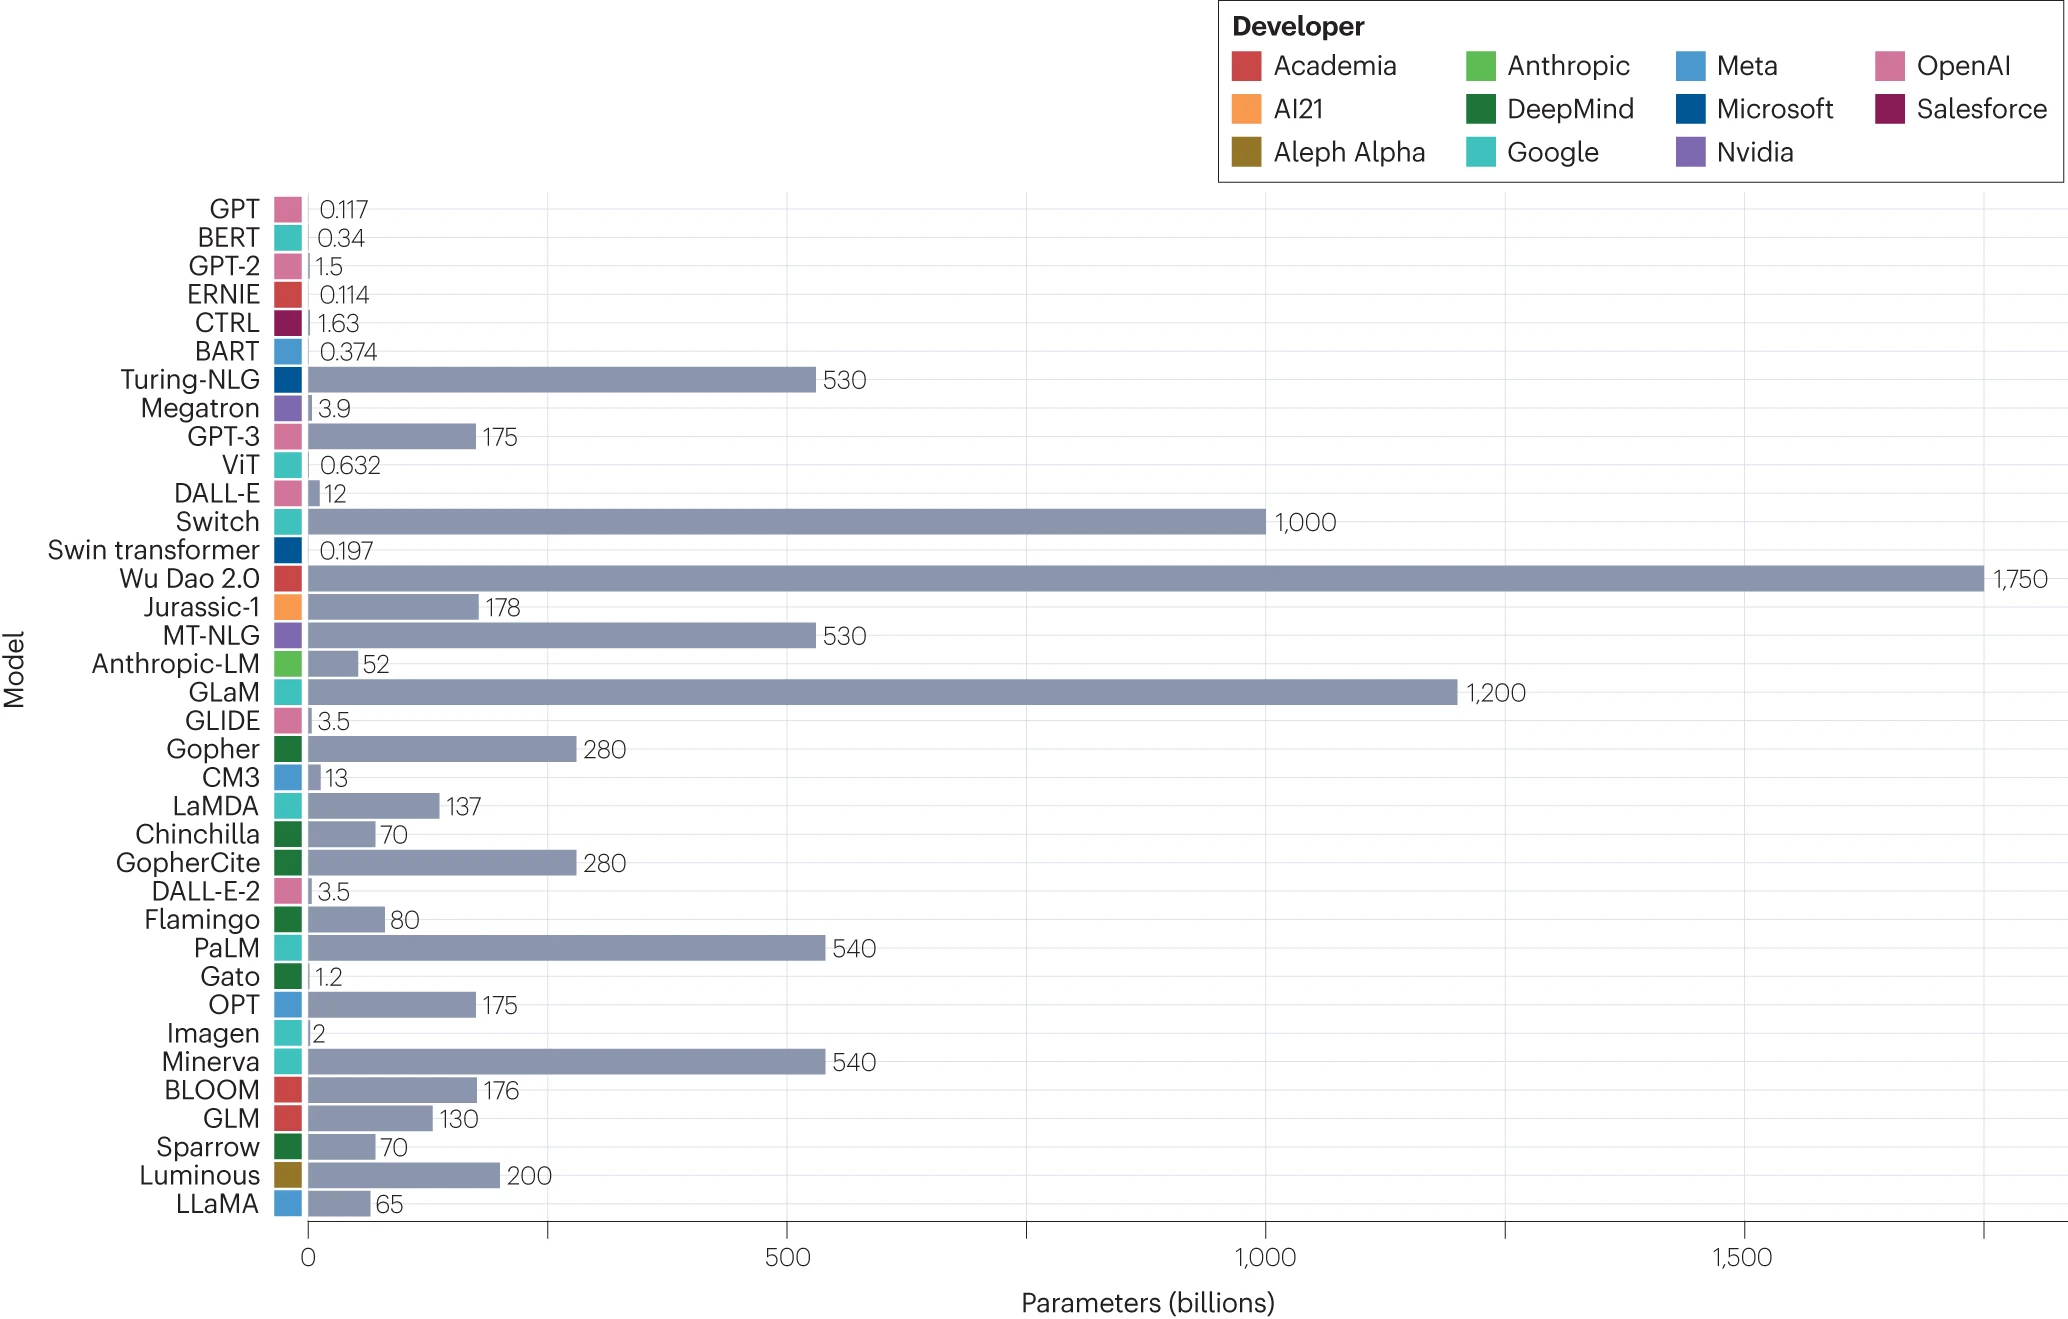
\includegraphics[width=1\textwidth]{img/recentllms.jpg}
    \caption{Comparativa de los billones de parámetros en distintos LLMs, \cite{thirunavukarasu_large_2023}}
    \label{fig:graficallms}
\end{figure}

\subsubsection{Funcionamiento de los LLM}

Ahora que se ha hablado de que es un LLM procede explicar la tecnología que estos tienen por debajo, los transformadores, una tecnología presentada por Google en 2017. Esta tecnología resulto revolucionaria en el campo, dejando obsoleta rápidamente a los métodos que se empleaban para realizar predicciones en lenguaje natural antes de su aparición.

En esencia los transformadores se basan en la arquitectura codificador-decodificador en la que también se basan otras inteligencias artificiales. Esta arquitectura consiste en, dos componentes principales, el codificador y el decodificador (en la figura \ref{fig:coddecod} se observa una representación de esta arquitectura). 

Un codificador no es más que un elemento matemático que convierte los datos de entrada en una representación matemática de los mismos, generalmente un vector, también llamada "hidden state". Por otra parte el decodificador recibe esa representación matemática de los datos de entrada y, según la tarea que se quiera realizar, traduce esa representación para ser parecida a aquella que fue introducida con el cambio deseado, como la traducción de un texto conservando su significado. En ambos elementos su funcionamiento depende enteramente de la tarea a realizar.

\begin{figure}[h]
    \centering
    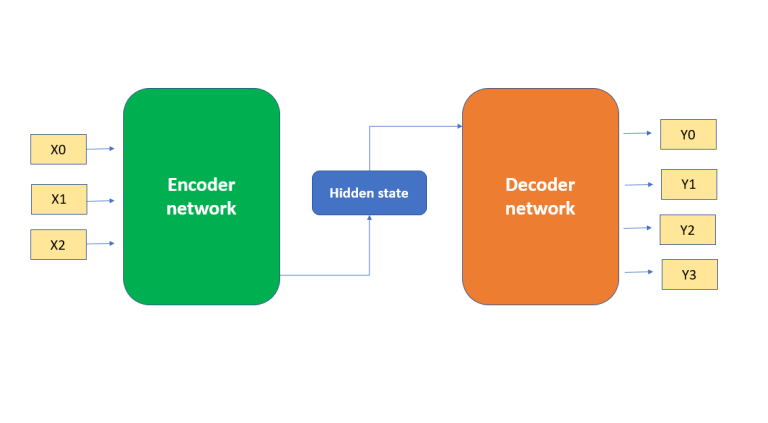
\includegraphics[width=1\textwidth]{img/encoder-decoder-architecture.png}
    \caption{Esquema de la arquitectura codificador-decodificador, \cite{kumar_demystifying_2024}}
    \label{fig:coddecod}
\end{figure}

Los LLM se basan en esta arquitectura. Estos modelos funcionan mediante el proceso de embedding para ''entender'' las relaciones entre fragmentos de texto llamados tokens (en la figura \ref{fig:llmarch} se puede ver un esquema del funcionamiento de la arquitectura subyacente a los LLMs).

Primero se debe dividir el texto de entrenamiento en fragmentos más pequeños (el tamaño de cada fragmento dependerá de la tarea). Estos fragmentos serán los llamados tokens que son representados en el modelo por embeddings. Un embedding es la representación vectorial del token en la que cada dimensión del vector representa un aspecto nuevo relacionado con el ámbito que está aprendiendo el modelo.

Este proceso de embedding tiene lugar en el codificador. Esta forma de codificación resulta especialmente eficiente en grandes volúmenes de datos, prueba de ello es la gran mejora de rendimiento en LLMs con respecto a otros modelos de inteligencia artificial a la hora de realizar tareas con textos en lenguaje natural. Dos vectores cercanos según técnicas matemáticas como la similitud del coseno o la distancia euclidiana se entienden cómo información relacionada para el LLM.

Cuando se genera una petición del usuario al modelo, se genera un embedding de la petición, los embeddings de los datos de entrenamiento más cercanos serán los que considere cómo posible respuesta.

Otro componente importante son los llamados mecanismos de atención, que capturan la información anterior y posterior al componente que se analiza para entender la información en su contexto y filtrar información poco relevante  manteniendo relaciones semánticas y contextuales entre palabras, y ofrecen otra ventaja importante a la hora de competir con otros modelos que no emplean estas tecnologías. Estos mecanismos de atención se encuentran tanto en el codificador como en el decodificador.

\begin{figure}[h]
    \centering
    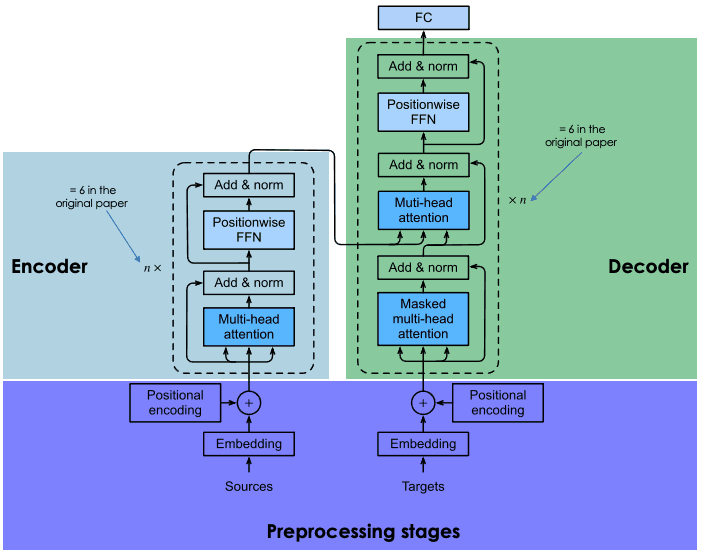
\includegraphics[width=1\textwidth]{img/llmarch.png}
    \caption{Esquema de la arquitectura de los transformadores en LLMs, \cite{javier_canales_luna_what_2023}}
    \label{fig:llmarch}
\end{figure}

\subsection{Entrenamiento de LLMs}

Es importante conocer ahora cómo estos modelos se entrenan ya que un modelo no entrenado no podría disponer de la información necesaria para aportarnos la información requerida.

El entrenamiento de un LLM cuenta de dos fases, el Pre-training y el Fine-tuning.

La fase de  pre-training es el paso inicial del entrenamiento, donde al modelo se le introduce una enorme cantidad de información en forma de tokens teniendo cómo objetivo que el modelo tenga un conocimiento general de la información proporcionada, este proceso es enormemente costoso en cuento a potencia de cálculo cómo en cuento a tiempo dependiendo de la magnitud del proyecto. Esta etapa es, por lo tanto, la más costosa económicamente siendo este el motivo por lo que hay pocos modelos open-source ya que estos requieren una enorme inversión inicial.

En el estado del arte del entrenamiento en LLMs se encuentra, entre otras técnicas, el fine tuning, una metodología en la que el modelo ya entrenado ve, al igual que el fine-tuning, su rendimiento optimizado, esta vez siendo mejorado para que siga las instrucciones presentes en los prompts de manera más efectiva

El paso de fine-tuning consiste en refinar un modelo preentrenado (que haya pasado la fase de pre-training) y, por lo tanto, ya goce de un conocimiento general de las relaciones contextuales y semánticas de los datos de entrenamiento y ''ponerlo a punto'' especificando su conocimiento a datos más específicos, haciendo que funcione mejor en casos más concretos como, por ejemplo, los datos de una clínica especializada en cardiología. Esta mejora está más pensada cómo una forma de mejorar el conocimiento previo más que una manera de expandirlo.


\subsection{Parámetros de interés en un LLM}

Los parámetros en LLMs comprenden tanto la arquitectura del modelo, es decir, la programación subyacente que hace que todo funcione, el tamaño del modelo, los datos de entrenamiento y los hiperparámetros.
Los hiperparámetro en inteligencia artificial son variables de configuración del modelo empleadas para controlar el proceso de aprendizaje del mismo e influenciar en los resultados.
Los hiperparámetros importantes en LLMs comprenden la temperatura, top p, longitud del token, tokens máximos, tokens de parada entre muchos otros que escapan el alcance de este proyecto.

\subsubsection{Temperatura}

La temperatura controla la aleatoriedad de las respuestas del modelo, dicho con otras palabras, controla su creatividad a la hora de explorar respuestas. Un modelo con una temperatura baja generará respuestas mas deterministas y fáciles de predecir siendo también más conservadoras con sus respuestas por lo que si se necesita una respuesta precisa con poca tolerancia a la creatividad y fallos es importante mantener una temperatura baja.

\subsubsection{Top-p}

El top-p, también conocido por nucleus sampling o muestreo de núcleo en español, es otro hiperparámetro que controla la aleatoriedad del modelo definiendo un límite que los tokens tienen que superar para ser considerados como respuesta del modelo. Después se seleccionará aleatoriamente una respuesta de entre todas las que hayan superado el umbral seleccionado. 

\subsubsection{Longitud de token}

La longitud de token es simplemente el número de palabras o caracteres que componen los tokens con los que trabaja el modelo. Este valor depende enteramente del propósito del modelo y de los datos de entrenamiento ya que una longitud de token muy pequeña puede hacer que se pierda contexto importante en la salida de los datos mientras que, por el contrario, tokens demasiado grandes harán que el modelo considere información poco relevante para la tarea que se espera que realice.

\subsubsection{Límite máximo de tokens}

El límite máximo de tokens es el número máximo de tokens que el modelo generará y procesará al mismo tiempo. Cuanto mayor sea este máximo, más coherente será la salida, pero con el coste de ser también más computacionalmente costosa. Este valor se definirá según el objetivo del modelo y de las limitaciones del hardware disponible.

\subsubsection{Tokens de parada}

Los tokens de parada son simplemente la longitud de la respuesta que el modelo diseñará. Al igual que el límite de tokens un mayor valor supone un mayor coste computacional. Si este valor se fija en 1 la respuesta se limitará a una frase, mientras que si aumenta a 2 esta consistirá en como mucho un párrafo.

\cite{jakindah_top_2023}

\subsection{Prompts}
Un prompt es la manera que tiene el usuario para interactuar con el modelo mediante la creación de instrucciones en lenguaje natural que se le pasan al modelo para que tras los cálculos nos ofrezca el output deseado.

El output depende en gran parte del prompt así cómo de los datos de entrenamiento y los parámetros del modelo,que serán explicados posteriormente.

El objetivo del prompt es aportar al modelo la información y el contexto necesario para que pueda ofrecer la respuesta deseada. Las distintas técnicas para refinar un prompt que ofrezca el resultado deseado se las conoce como prompt engineering. En el siguiente apartado hablaremos más a fondo de ellas con un enfoque a su aplicación en la medicina y las ciencias de la salud.

\subsubsection{Prompt Engineering}

El prompt engineering es crucial a la hora de trabajar con modelos grandes de lenguaje y obtener los resultados deseados. En el ámbito sanitario un prompt puede definir escenarios reales y detallados con la mayor cantidad de información posible o especificando lo más concretamente posible la información que se quiera obtener de los datos de entrada .

Para reafirmar la potencia que tiene esta técnica en datos médicos, ChatGPT un chatbot consiguió mediante el uso de prompts adecuados llegar al nivel de aprobar el examen de licencia médica de Estados Unidos (USMLE) demostrando un gran nivel en sus razonamientos \cite{thirunavukarasu_large_2023}.

A la hora de diseñar prompts tenemos varios tipos, los "Few-Shot" o los "Zero-shot" son dos de ellos. 

El "Zero" presente en el nombre quiere decir que el prompt será pedirle al modelo una tarea y no se le proporcionará un ejemplo. Aunque esto en un primer vistazo parezca fútil o de poca utilidad pero este tipo de prompts resultan muy útiles para diversas tareas cómo la traducción de textos sin realizar ningun tratamiento o tarea específica al texto de entrada.

Los "Few-shot" prompts por su parte se diferencian de los "zero-shot" prompts en que contienen un ejemplo para ayudar al modelo a efectuar la tarea aunque tampoco sea la tarea aquella para la que el modelo haya sido entrenada.

Antes de hablar más a fondo de otros tipos de prompts es importante que se definan los niveles de complejidad que puede llegar a tener un prompt.

Los prompts de primer nivel simplemente consisten en preguntas muy simples sin refinar, como por ejemplo ¿Qué es el Covid-19?
Los de segundo nivel consisten en ofrecer un contexto al modelo para mejorar el prompt; podría ser: "Eres un profesor de ingeniería de la salud de la universidad de Burgos y yo soy tu estudiante ¿Me podrías enseñar sobre el Covid-19?"
Por otra parte, los de tercer nivel también agregan ejemplos a los mismos siguiendo la linea fewshot. Podría consistir en aportar un abstract de un artículo relacionado con el Covid-19 y añadir el prompt de nivel 2 para obtener uno de nivel 3. Para finalizar los niveles, los de cuarto nivel permite al modelo descomponer la solicitud en componentes.

Otro método que ha demostrado obtener buenos resultados a la hora de crear prompts son los llamados prompts estructurados. Estos consisten en aportar información extra en el prompt para dar forma a nuestro resultado deseado, Hay muchas estrategias que ayudan a esto, suelen estar denominadas en siglas fáciles de recordar que indican de que información se compondrá nuestro prompt.

Las estrategias de prompts estructurados más conocidas son:

\begin{itemize}
    \item APE: Action, Purpose, Expectation
    \item RACE: Role, Action, Context, Expectation
    \item COAST: Context, Objective, Actions, Scenario, Task
    \item TAG: Task, Action, Goal
    \item RISE: Role, Input, Steps, Expectation
    \item TRACE: Task, Request, Action, Context, Example
    \item ERA: Expectation, Role, Action
    \item CARE: Context, Action, Result, Example
    \item ROSES: Role, Objective, Scenario, Expected Solution, Steps
    
\end{itemize}
\cite{edi_hezri_hairi_2_2023}


Por último Se hablará de los prompts iterativos. Estos son aquellos que el propio LLM ayuda en su creación ya que se creará un prompt inicial y se le pedirá al modelo que vaya refinando el prompt, expresándole los objetivos que se quieren obtener. Puede que se necesiten varias iteraciones para obtener un prompt lo suficientemente bueno, que obtenga información precisa y detallada que incluso puede superar las expectativas iniciales del usuario.

\subsubsection{Malos Prompts}

Se podrían considerar como malos prompts aquellos que no generen el resultado deseado o generan resultados de información falsa. Esto no siempre es culpa del prompt ya que un entrenamiento inadecuado puede conllevar al mismo resultado.

Malos prompts por lo general son aquellos poco preciosos o engañosos. Un prompt poco preciso puede llevar al modelo a generar una respuesta poco precisa o generar una respuesta que no satisfaga al usuario, ya que puede haber una cantidad insondable de información. Por ejemplo, "¿Que enfermedad puede tener mi paciente?" sin proporcionar más información, un modelo podría indicar que necesita más información, o citar cierto número de enfermedades que pueda padecer.

Los prompts engañosos son en los que se introduce un sesgo como por ejemplo "¿Por qué los hospitales deberían aumentar el número de camillas?" Cuando en realidad puede que la respuesta correcta sea que no deban hacerlo por los recursos de los que dispone al introducir el sesgo en la pregunta se pude recuperar respuestas engañosas. 

Otro tipo de prompts malos y engañosos son en los que se añade información falsa cómo por ejemplo "¿Qué hongo causa el Covid-19?" Aunque es cierto que muchos modelos detectan este error, puede que un modelo más simple intente buscar alguna información que concuerde con el prompt.

\cite{heston_prompt_2023}

\subsection{Usos comunes de los LLM}

En esta sección se expondrán áreas en las que los LLM podrían aportar información interesante. El campo de la medicina tendrá su propio apartado ya que, por el objetivo de la titulación y de este trabajo, es el campo que más interés posee por lo que se abordará en mayor profundidad.
\subsubsection{Ciberseguridad}

Un LLM puede ser entrenado con un gran volumen de datos de ciberseguridad cómo ataques pasados o consejos que publiquen expertos en el campo para poder predecir y anticiparse a futuros ataques. Este campo resulta especialmente interesante debido al componente humano de los riesgos en linea ya que estos modelos analizan el lenguaje natural como ya se ha explicado con anterioridad. 
\subsubsection{Educación}

Los LLM se pueden emplear para diseñar material educativo personalizado para cada usuario: haciendo hincapié en los apartados en los que más fallos se cometan, empleando la función de memoria con la que cuentan muchas aplicaciones, siguiendo la evolución del usuario.
\subsubsection{Atención al cliente}

Los LLM entrenados con la información de una empresa pueden ofrecer ayuda a las consultas que los clientes puedan tener sobre la misma así cómo ofrecer recomendaciones o consejos. Estas funcionalidades se pueden acentuar aún más empleando las técnicas de RAG.
\subsubsection{Traducción y localización}

Estos modelos también son potentes para salvar la barrera entre idiomas no sólo por ser capaz de traducir el texto, si no por ser capaz de localizarlo, es decir, adaptar el lenguaje para hacerlo más claro para el receptor que hable un idioma ajeno al original adaptando expresiones y modismos que pudieran resultar confusos si fuesen traducidos literalmente.
\subsubsection{Creación de contenido}

Otro campo en el que actualmente está destacando esta tecnología es en la creación de guiones iniciales, guías o bocetos para el desarrollo de libros, artículos, trabajos etc. Aunque el trabajo creativo siga estando de mano del usuario, los LLM han probado ser una herramienta poderosa para guiar la creatividad del usuario y ayudarlo en la creación del producto final aumentando el rendimiento y la productividad.
\subsubsection{Análisis de datos}

En el campo del análisis de datos se destaca la capacidad de los modelos de generar información de los propios datos en diferentes formatos ya sea audio, vídeo o texto, extrayendo la información relevante, generando resúmenes o respondiendo preguntas de la información contenida en los archivos de interés.

\cite{jesse_sumrak_7_2024}

\subsection{Empleo de los LLMs en medicina}

El objetivo de este trabajo es dar una demostración de una posible aplicación de esta herramienta en un campo tan crucial para la sociedad como es la medicina. La aplicación propuesta es un buen ejemplo y en esta sección se explorarán mas aplicaciones y avances.
En primer lugar tenemos el procesado de lenguaje natural más convencional a la hora de interpretar datos y emitir diagnósticos. Una versión del modelo PaLM 2 de Google aplicada a la medicina conocida como Med-PaLM 2 ha conseguido funcionar a un altísimo nivel, siendo equiparado al nivel de un clínico experto incluso en algunos casos llegando a superarlos en campos como la empatía con el paciente.

Aunque la información anterior da la visión de que la inteligencia artificial puede sustituir a los médicos profesionales a la hora de emitir un diagnóstico esto no es así. Los modelos tienen limitaciones como datos incompletos o directamente perjudiciales para el paciente que pueden generar respuestas erróneas y peligrosas. Aunque todavía no puedan sustituir a un médico especialista, los LLM ayudan a agilizar el proceso de diagnóstico y, por lo tanto, aumentan la eficiencia del sistema de salud.

Otro campo en el que los LLM parecen hacerse hueco en el mundo de la medicina es en la gestión de los recursos hospitalarios, el uso de camas, la medicina de triaje, etc. Pueden ofrecer soluciones rápidas y efectivas cuando más se necesita siempre que esté alimentado con los datos de los recursos de los que el hospital dispone.

Otra posible aplicación son los chatbots especializados en asistencia médica. Aunque este campo requiera mucha información ya que en la actualidad dejar a un modelo grande de lenguaje decidir un tratamiento o proveer asistencia médica a enfermos puede ser peligroso por las limitaciones actuales, se abre un campo de estudio muy interesante, el desarrollo de asistentes médicos virtuales entrenados en datos especializados. Mediante el proceso de RAG se puede incluir los datos específicos del paciente en cuestión, proporcionando ayuda especializada y revisada por profesionales médicos aliviando la carga de muchos profesionales médicos solventando posibles problemas de colapsos en la sanidad. Esto podría haber sido una gran ayuda en la época de la pandemia y merece la pena investigar en ello por posibles situaciones similares en un futuro.

\cite{kim_chatgpt_2023}, \cite{clusmann_future_2023}

\subsection{Desventajas y malos usos de los LLMs}

Aunque los LLM tengan grandes ventajas, puede existir malos usos, no solo por prompts malos o insuficientes que generen resultados indeseados o pobres, si no por su empleo en actividades inmorales como el plagio (figura \ref{fig:prosandcons}). Aunque los beneficios son mayores, ignorar los riesgos sería caer en un error grave así cómo lo sería obviar los grandes avances que esta tecnología está generando y promete generar en un futuro.

\begin{figure}[h]
    \centering
    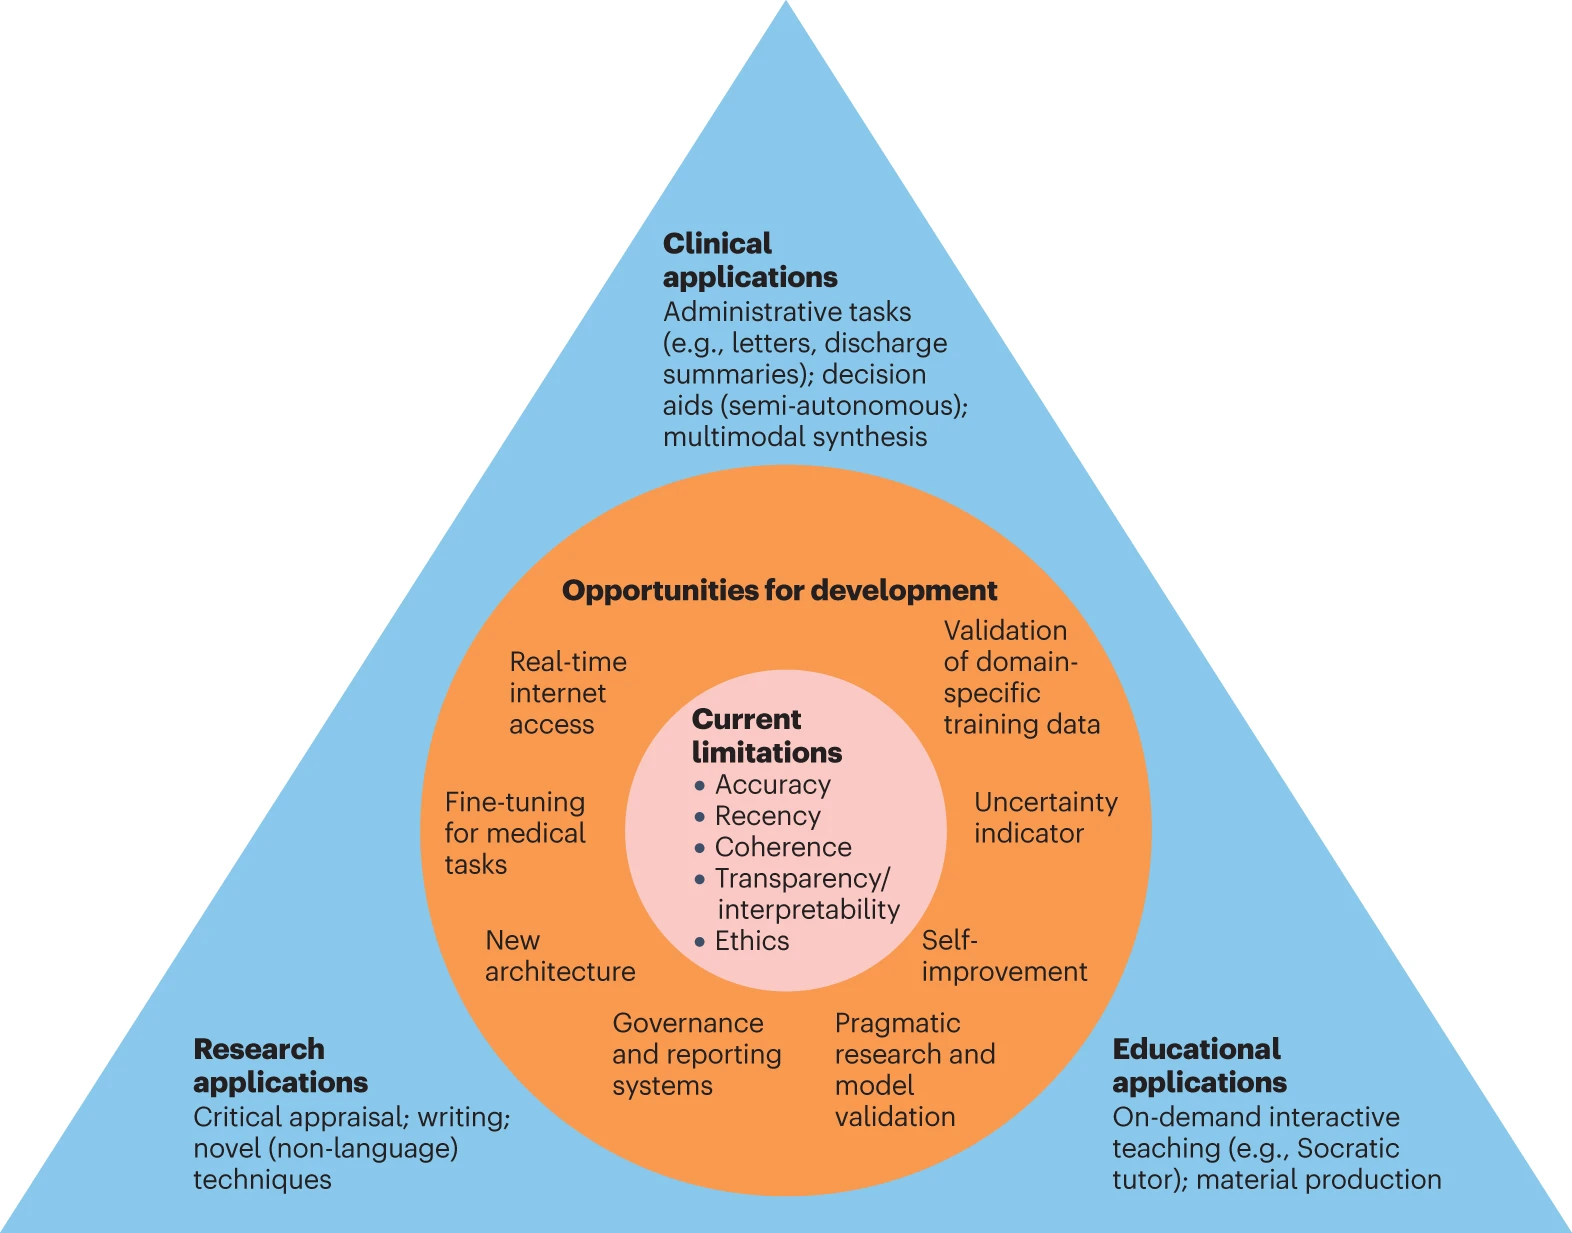
\includegraphics[width=1\textwidth]{img/pros_and_cons.jpg}
    \caption{Algunos beneficios y limitaciones de los LLM, \cite{thirunavukarasu_large_2023}}
    \label{fig:prosandcons}
\end{figure}

\subsection{Diferentes LLMs}

Actualmente y al ser una tecnología nueva que está demostrando grandes resultados, hay multitud de modelos. A continuación se expone un repaso de los más influyentes. En la tabla \ref{tab:tablellm} se puede consultar información relevante de los mismos.

\begin{table}[]
\begin{tabular}{lllll}
\textbf{Nombre del Modelo}     & \textbf{Desarrolladora}                & \textbf{Acceso}           &  &  \\
GPT                     & OpenAI                          & API              &  &  \\
Gemini                  & Google                          & API              &  &  \\
Gemma                   & Google                          & Open             &  &  \\
Llama 3                 & Meta                            & Open             &  &  \\
Vicuna                  & LMSYS Org                       & Open             &  &  \\
Claude 3                & Anthropic                       & API              &  &  \\
Stable Beluga           & Stability AI                    & Open             &  &  \\
StableLM 2              & StabilityAI                     & Open             &  &  \\
Coral                   & Cohere                          & API              &  &  \\
Falcon                  & Technology Innovation Institute & Open             &  &  \\
DBRX                    & Databricks and Mosaic           & Open             &  &  \\
Mistral 8x7B and  8x22B & Mistral AI                      & Open             &  &  \\
XGen-7B                 & Salesforce                      & Open             &  &  \\
Grok                    & xAI                             & Chatbot and Open &  & 
\end{tabular}
\caption{Principales LLMs en la actualidad, \cite{harry_guinness_best_2024}}
\label{tab:tablellm}
\end{table}

\subsubsection{GPT – OpenAi}

Posiblemente el modelo más reconocido a día de hoy, presente en una aplicación que se ha vuelto de uso casi rutinario, ChatGPT. Su nombre proviene de las siglas de Generative Pre-trained Transformer, cuenta con más de 175 mil millones de parámetros en su versión GPT-3, los cuales aumentan en sus versiones posteriores, GPT-3 Turbo, GPT-4 y GPT-4 Turbo. En la actualidad muchas empresas emplean sus servicios como por ejemplo Microsoft o la app de idiomas Duolingo.

\subsubsection{Gemini- Google}

 De menos parámetros, unos 3 mil millones, está diseñado para operar en distintos dispositivos y con diferentes tipos de inputs ya sean audio, texto, vídeos o código. Actualmente su uso principal reside en las aplicaciones de Google.
 
\subsubsection{Llama 3 – Meta}

EL modelo de la gigante tecnológica Meta destaca por tener, actualmente en entrenamiento, un modelo de 400 mil millones de parámetros, una cantidad insondable para muchas empresas. Aparte tiene dos opciones más pequeñas de 70 y 8 mil millones de parámetros. Es de código abierto para usos comerciales y de investigación, por lo que muchos modelos aquí listados usan Llama 3 cómo su base.

\subsubsection{Mistral – Mistral}

Sus modelos destacan por su relativamente pequeño tamaño y por la optimización que estos tienen, lo cual les permite rivalizar a otros modelos más grandes y usados por grandes empresas. La optimización de parámetros le permite al modelo ejecutarse más rápido y en un hardware mucho menos potente que sus competidores.


\section{proceso de RAG}
\subsection{Introducción al RAG}

Al trabajar con modelos grandes de lenguaje, muchas veces la respuesta que se obtiene muestra la falta de información no contenida en los datos de entrenamiento. Para aumentar la calidad de nuestros resultados se ha implementado una tecnología llamada RAG (Retrieval Augmented Generation) para aumentar y acotar, con los recursos ya existentes del modelo, la información que posee, alimentándolo con los datos que puedan resultar de interés para la tarea.

El principal beneficio de emplear técnicas de RAG en LLMs consiste en poder realizar consultas precisas a los datos aportados por el usuario. Esto en empresas cómo en sectores sanitarios es muy útil ya que si el repositorio de información empleada para el proceso de RAG es una base de datos, podríamos interactuar con ellos en tiempo real realizando consultas de forma cómoda en lenguaje natural. El profesional sanitario con mínimos conocimientos informáticos podría interactuar con la base de datos de manera precisa y sin riesgos de que tome información de recursos poco fiables o que no tengan que ver con la tarea a realizar.

En la figura \ref{fig:ragrpoc} se puede ver una representación gráfica del proceso de RAG

\begin{figure}[h]
    \centering
    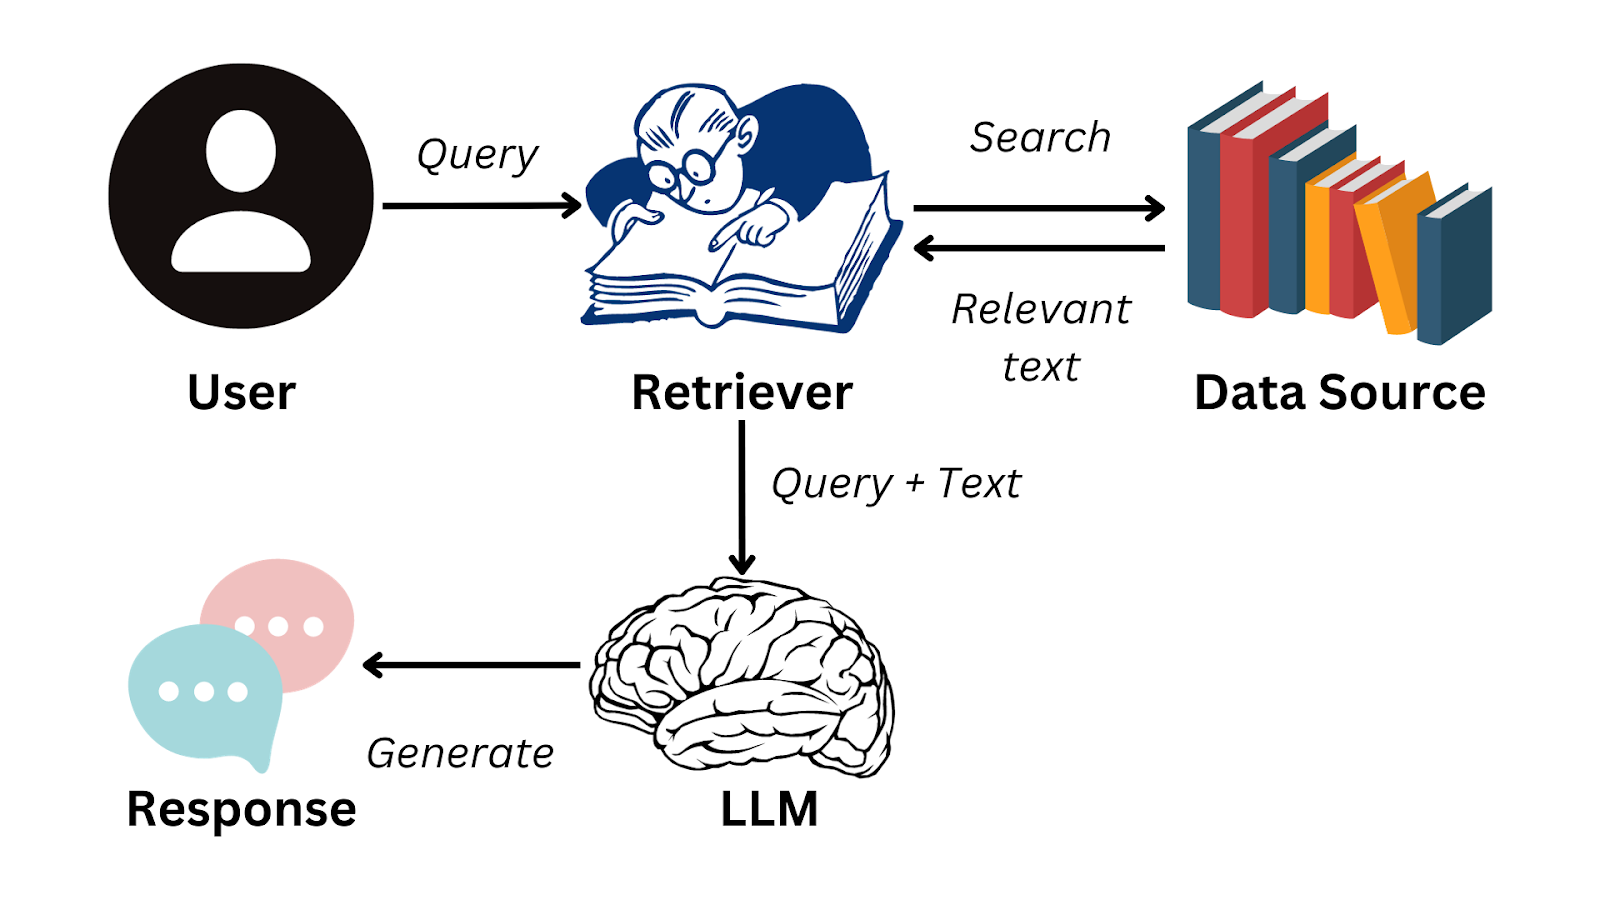
\includegraphics[width=1\textwidth]{img/ragproc.png}
    \caption{Proceso de RAG, \cite{natassha_selvaraj_what_2024}}
    \label{fig:ragrpoc}
\end{figure}


\subsubsection{Descripción del proceso de RAG}

El primer paso, evidentemente, consiste en identificar en que datos se quiere que se especialice el modelo y recuperarlos, el formato puede ser muy diverso, desde vídeos, CSV, PDFs, páginas web, bases de datos etc.

Después, se debe realizar un proceso de desmenuce, dividir la información de interés en chunks (trozos) que contengan diferente información relacionada para aumentar la eficiencia sin procesar documentos enteros. Una vez obtenidos habrá que hacerlos pasar por el proceso de embedding, generando embeddings por cada chunk, que es almacenado en una base de datos vectorizada.

Una vez realizado los embeddings de los datos de interés hay que esperar a la petición del usuario y generar un embedding de esta última también. Después se comparan las distancias entre el embedding de la petición y se devuelven los embeddings de los chunks más cercanos según la similitud de cosenos junto a los de la petición.

Y por último, teniendo los chunks relevantes a la petición junto a la misma, se insertan ambos en un LLM que generará una respuesta empleando la petición junto a los datos relevantes a la misma.

\section{PubMed}

PubMed es una página web gratuita fundada en 1996 que contiene abstracts de  literatura biomédica así cómo los enlaces para recuperar los textos completos. Los artículos empleados para la elaboración de este trabajo así como los abstracts empleados para el proceso de RAG de la aplicación han sido recuperados de PubMed.

Los recursos de PubMed tienen varios orígenes.

\subsection{MEDLINE}

El componente principal de PubMed. La literatura científica aquí presente consiste en citas de revistas científicas indexadas con MeSH, unos términos especiales para facilitar la navegación en literatura biomédica.

\subsection{PubMed Central}

El segundo componente de PubMed, contiene artículos completos de revistas científicas revisados y seleccionados por la Biblioteca Nacional de Medicina (NLM)
\subsection{Bookshelf}

El componente final de PubMed, contiene libros, informes, bases de datos y otros documentos relacionados con la biomedicina.

\cite{pubmed_1996}

\section{COVID-19}

El COVID-19 es un virus causante del síndrome agudo respiratorio severo, que originó una pandemia declarada cómo tal el 11 de Marzo por la Organización Mundial de la Salud (OMS). Por el peligro inminente que supuso y el impacto mundial que causó, generó en la época de pandemia y posteriormente, una gran cantidad de datos.

\cite{habas_resolution_2020}

\capitulo{4}{Metodología}

\section{Descripción de los datos.}

Los datos con los que se trabaja son abstracts de papers científicos recuperados de PubMed, 
Una descripción más detallada de los datos se encuentra en el anexo D.


\section{Técnicas y herramientas.}

Esta parte de la memoria tiene como objetivo presentar las técnicas metodológicas y las herramientas de desarrollo que se han utilizado para llevar a cabo el proyecto.

\subsection{Python}

Python es un lenguaje de programación creado por Guido van Rossum en 1991, posee las siguientes características:

\begin{enumerate}
    \item Lenguaje interpretado o de script
    
    \item  Tipado dinámico

    \item  Fuertemente tipado

    \item  Multiplataforma

    \item  Orientado a objetos
    
\end{enumerate}

Se ha empleado python por sus librerías especializadas en inteligencia artificial de las que se hablará mas adelante y por su sintaxis clara y sencilla, para concer más información sobre el lenguaje python en español consultar el libro Python para todos \cite{gonzalez2011python}.

\subsection{LangChain}

LangChain es un marco para construir con modelos grandes de lenguaje (LLMs) mediante la conexión de componentes interoperables. LangGraph es el marco para construir flujos de trabajo agentivos controlables.

Destaca por ser fácil de empezar a usar sin sacrificar el potencial de escalada.

Entre muchas de sus aplicaciones se encuentran los retrievers, Las conexiones de datos y la infraestructura que necesitas para el retrieval de la información. Con los métodos integrados de ingestión y recuperación de LangChain, los desarrolladores pueden aumentar el conocimiento del modelo de lenguaje (LLM) con datos del usuario.

Otra prestación que ofrece LangChain, imprescindibles para el proyecto son los denominados data loaders, funciones que permiten cargar datos en el sistema para que puedan ser procesados por las distintas funcionalidades que ofrece LangChain.
LangChain ofrece una gran cantidad de recursos, se puede observar en la imagen \ref{fig:langchain}.

\begin{figure}[h]
    \centering
    \includegraphics[width=1\textwidth]{img/langchain.png}
    \caption{Prestaciones LangChain, reuperado de \cite{langchain_2022}}
    \label{fig:langchain}
\end{figure}

\subsection{Pytorch}

Pytorch es una librería de alto nivel en python que tiene dos funciones principales:

\begin{enumerate}
    \item Proveer de una clase tensor de alto rendimiento, muy útil para todas las costosas operaciones que se llevan a cabo en el ámbito del machine learning.
    
    \item  Definir un framework para el desarrollo de aplicaciones de inteligencia artificial.
\end{enumerate}

Para ver más información en \cite{pablo_huijse_heise_12_2022}

\subsection{Hugging Face}

Hugging Face es una plataforma y comunidad de aprendizaje automático (ML) y ciencia de datos que ayuda a los usuarios a construir, desplegar y entrenar modelos de aprendizaje automático.

Proporciona la infraestructura para demostrar, ejecutar y desplegar inteligencia artificial (IA) en aplicaciones en vivo. Los usuarios también pueden navegar por modelos y conjuntos de datos que otras personas han subido. A menudo se llama a Hugging Face el GitHub del aprendizaje automático porque permite a los desarrolladores compartir y probar su trabajo abiertamente. Para conocer más sobre HuggingFace \cite{ben_lutkevich_what_2023}

En este proyecto el uso de Hugging Face destaca por la posibilidad de emplear modelos de inteligencia artificial de manera gratuita, en este caso se ha empleado el modelo Mistral 7B para la generación de respuestas y el sentence-transformers/all-mpnet-base-v2 para la generación de embeddings.

\subsection{FAISS}

Por sus siglas, Facebook AI Similarity Search, o, en español, búsqueda por Similitud de IA de Facebook, se trata de una librería desarrollada por la empresa Meta que ayuda a la hora de realizar el proceso de RAG ya que permite buscar rápidamente elementos que son similares entre sí, más información se puede encontrar en la publicación original \cite{herve_jegou_faiss_2017}.

En este proyecto se han empleado las bases de datos vectorizadas que esta librería ofrece, prestando una gran ayuda a la hora de comparar la información vectorizada en el proceso de RAG.

\subsection{Google Colab}

Para la edición de código se ha empleado Google Colab, un entorno virtual que permite programar y ejecutar python, fue elegido por su opción de añadir la aceleración por hardware, T4 GPU al entorno de ejecución como se puede ver en la figura \ref{fig:acel}.

\begin{figure}[h]
    \centering
    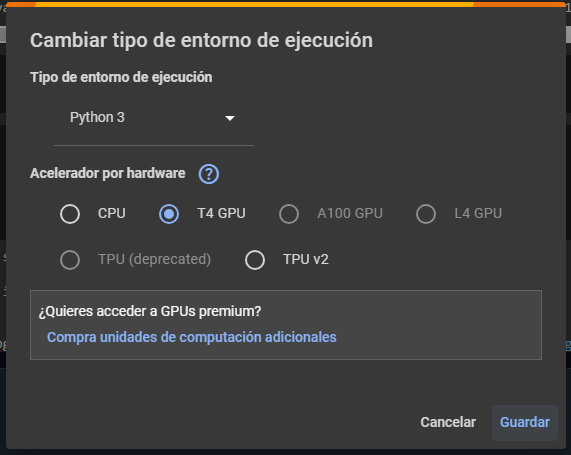
\includegraphics[width=1\textwidth]{img/aceleracion.png}
    \caption{Prestaciones LangChain, reuperado de \cite{retrieval}}
    \label{fig:acel}
\end{figure}

\subsection{Zube.io}

Zube.io es un gestor de proyectos que emplea metodologías ágiles como Kanban o Scrum. En este proyecto ha resultado útil para la planificación de tareas.

En el anexo A se puede encontrar un desglose detallado de cómo se ha empleado esta herramienta.

\subsection{Github}

GitHub es un gestor de repositorios en linea empleado fundamentalmente para la creación de código. Desde hace años resulta una herramienta indispensable para el desarrollo de software, permitiendo, entre otras cosas, la colaboración entre varios desarrolladores, el seguimiento del desarrollo mediante "issues" y la gestión de varios repositorios que pueden funcionar como portfolio o simplemente para almacenar código.

Todo el proyecto se encuentra público en el repositorio:\\
dlp1004/Aplicacion\_de\_chatbot\_con\_LLM\_y\_RAG\_para\_la\_gestion\_de\\\_informacion\_cientifica\_de\_COVID-19\_en\_PubMed

\subsection{Kaggle}

Kaggle es una comunidad centrada en la inteligencia artificial y el machine learning, tiene varias funcionalidades, entre ellas destaca la publicación de código, modelos y datasets, también se celebran en ella competiciones y discusiones sobre temas relacionados, para este proyecto su papel ha sido el de extraer los datos de entrenamiento, \cite{Anandhu_H_abstracts_2023}.

\subsection{Overleaf}

Overleaf es la herramienta en la que se está escribiendo toda esta documentación, se trata de un editor en linea de Latex, intuitivo y fácil de usar.

\subsection{ChatGPT}

Para tareas de traducción y redacción se ha empleado ChatGPT, otra herramienta de chatbot que emplea los LLMs GPT-3.5 y GPT-4, para más información sobre LLMs, dirigirse al capítulo 3 de esta memoria.

\subsection{Gradio}

Gradio es una librería diseñada para python que provee de un framework para realizar demos de interfaces para aplicaciones de machine learning, una ventaja de este paquete es que una interfaz de Gradio se puede integrar en notebooks de Python o presentarse como una página web.

Una interfaz de Gradio puede generar automáticamente un enlace público que puedes compartir con colegas, permitiéndoles interactuar con el modelo en tu computadora de forma remota desde sus propios dispositivos, lo que hace muy conveniente su utilización para una prueba de concepto.

Gradio también provee de servicios de Hosting permanente con su integración con los espacios de Hugging Face, lamentablemente este proyecto demanda una cantidad de gpu que escapa la disponible en el servicio de hosting gratuito.
\capitulo{5}{Resultados}

\section{Resumen de resultados.}

En este capítulo se incluirá un breve resumen de los resultados.

\subsection{Aplicación}

Cómo resultado del proyecto se ha desarrollado una aplicación de chatbot al que, tras incluirle una respuesta, buscará en una base de datos vectorizada y recuperará abstracts relacionados a la pregunta introducida, con esta información buscará responder a la cuestión previamente introducida por el usuario. Para su interacción con el usuario se ha desarrollado una interfaz gráfica en Gradio, en la imagen \ref{fig:guivacia} se puede observar dicha interfaz en su forma más básica, en la que no hay ninguna ejecución, se pueden distinguir un gran campo de texto donde se encontrará la respuesta proporcionada por el modelo, otro justo debajo mas pequeño, en este caso de input, dónde se introducirá la petición al modelo, para enviarlo habrá que presionar el botón de "Submit". Tras la ejecución se verá como en la imagen \ref{fig:guirellena}, en este caso tienen sentido los tres botones que se observan que serían, de izquierda a derecha:

\begin{enumerate}

    \item Retry: vuelve a mandar al modelo el último prompt enviado para obsevar distintos resultados, como este modelo está parametrizado para "alucinar" poco es muy probable que la respuesta sea la misma o tenga diferencias poco significativas.
    
    \item Undo: elimina la ultima iteración del modelo, es decir, del registro mostrado por pantalla se dejan de mostrar la ultima petición y el ultimo resultado.
    
    \item Clear: elimina todo el historial de chat.
    
\end{enumerate}

\begin{figure}[h!]
    \centering
    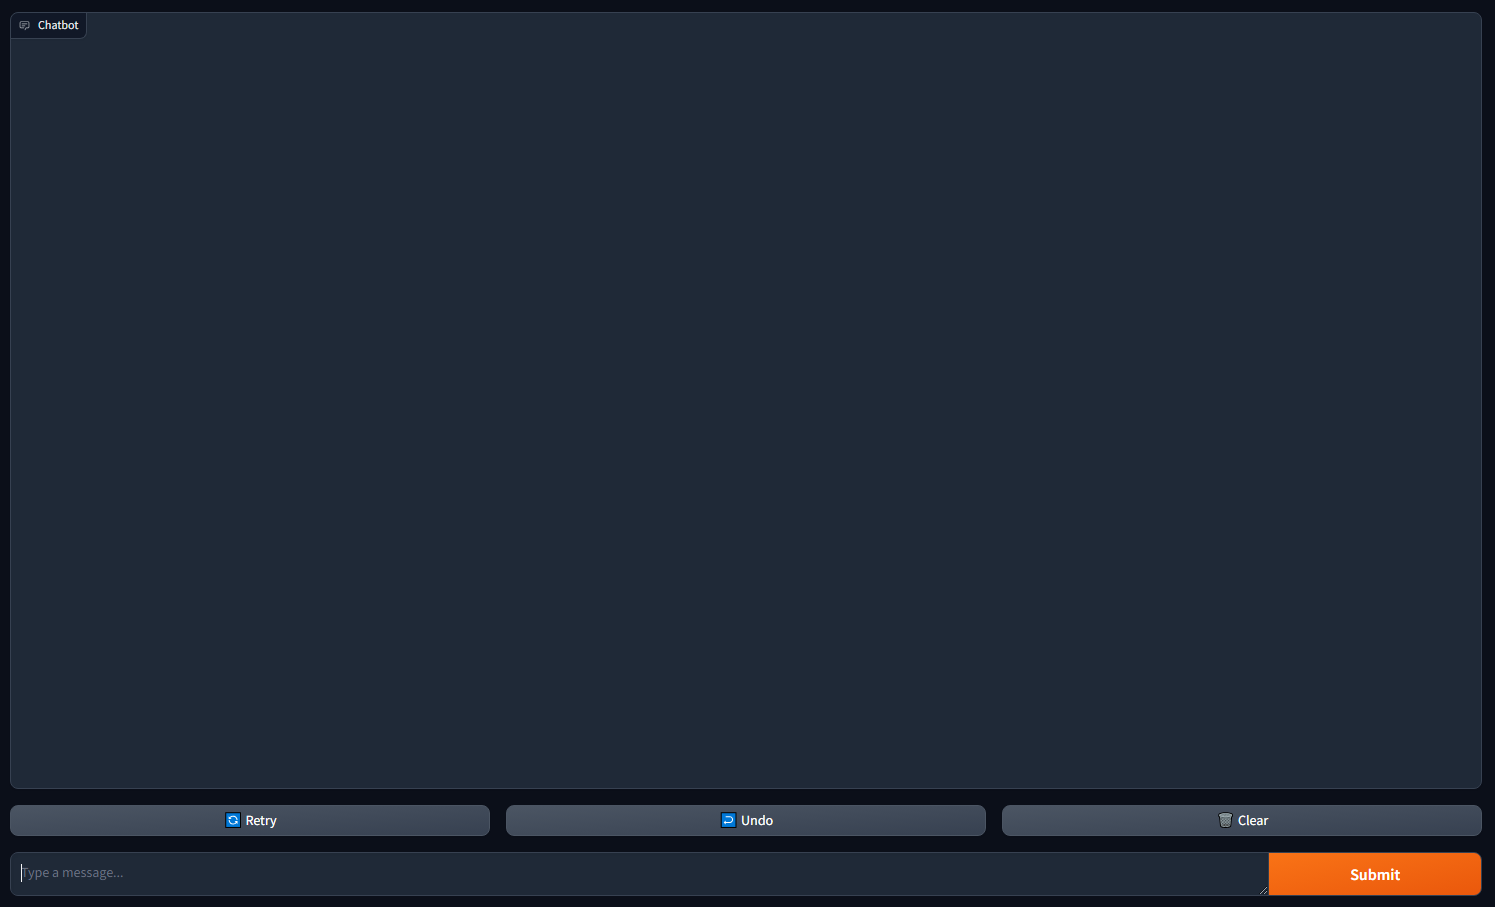
\includegraphics[width=1\textwidth]{img/guivacia.png}
    \caption{Interfaz gráfica de usuario}
    \label{fig:guivacia}
\end{figure}

\begin{figure}[h!]
    \centering
    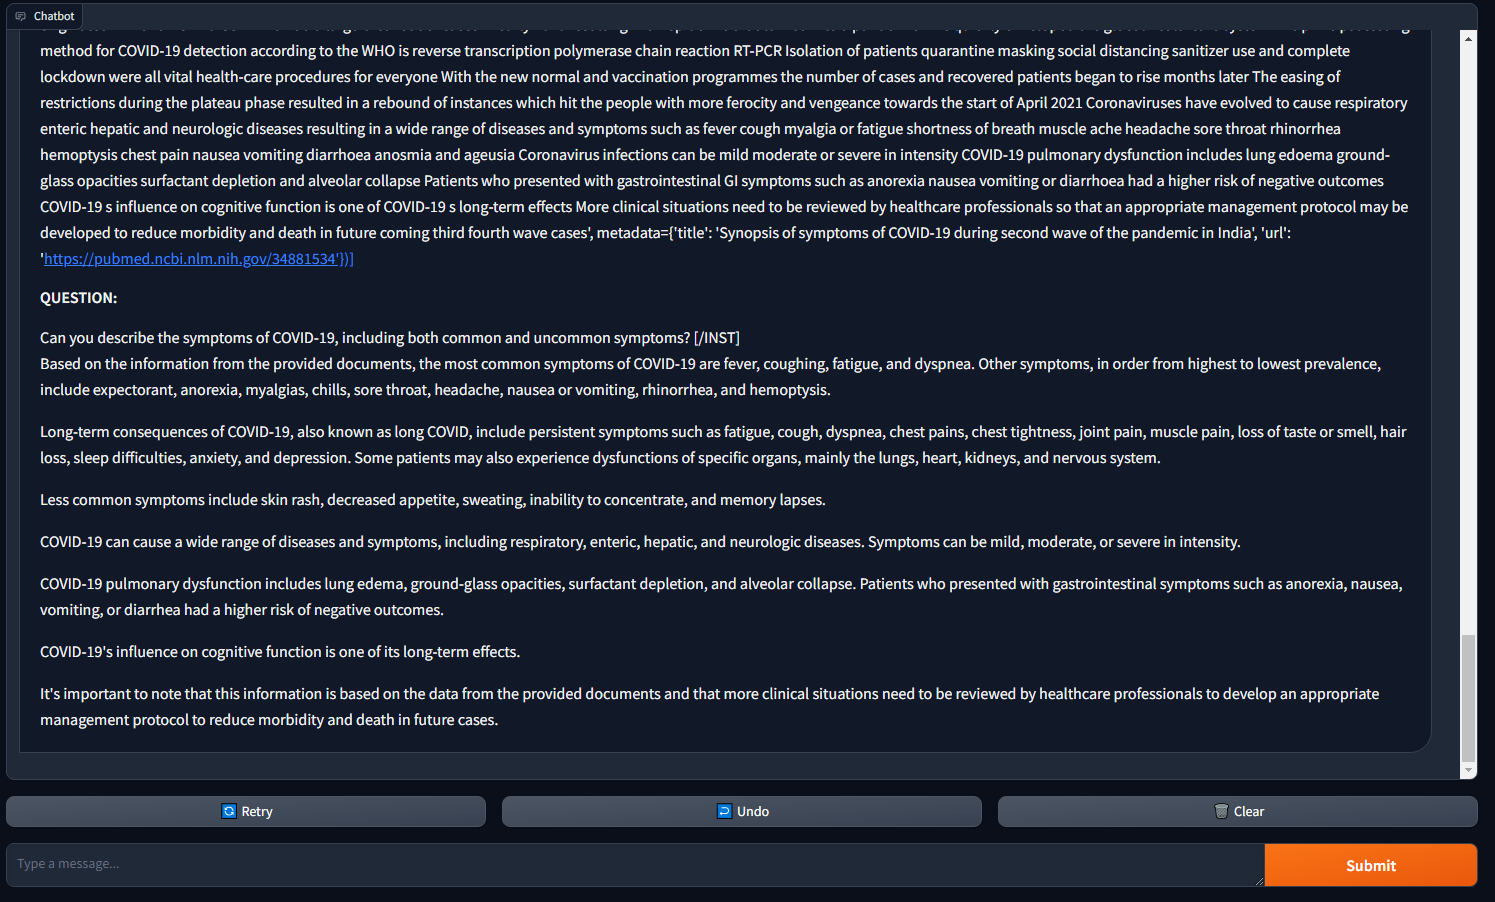
\includegraphics[width=1\textwidth]{img/guirellena.png}
    \caption{Interfaz gráfica de usuario tras una ejecución}
    \label{fig:guirellena}
\end{figure}

\FloatBarrier

\subsection{Salidas del programa}

En el anexo G se ha realizado una validación exhaustiva de diferentes salidas del programa, sin embargo en esta sección se observarán ejemplos distintos de las distintas posibles salidas.

\subsubsection{Salida sin retrieval}

En este ejemplo se propone un prompt que no tiene nada que ver con el tema en el que el programa está especializado, es decir, Covid-19. Se puede observar como no devuelve ningún abstract (el apartado de contexto está vacío, sólo se encuentra un []) ya que no hay ninguno en la base de datos vectorizada que sobrepase el threshold impuesto en la parametrización del retriever.

Prompt: What's the sun's mass?

Contexto: []

Salida: [INST] Instruction: You are an expert in microbiology. Please answer the question based ONLY on your knowledge of abstracts from a series of articles in this prompt don't use information of any other kind, if there were not any articles passed in this prompt just indicate that:
[]

QUESTION:
What's the sun's mass? [/INST]
I'm an expert in microbiology and I don't have the ability to directly answer questions about the mass of the sun based solely on the information from the abstracts provided in this prompt. The abstracts do not contain any information about the mass of the sun.

\subsubsection{Salida con retrieval específico}

En este caso se le hará una pregunta muy específica de la que hay pocos artículos que hablen, el retrieval será escueto ya que se prefiere recuperar poca información a recuperar bastante información que no tiene que ver con el tema ya que, en el ámbito biomédico, puede tener consecuencias fatales.

Prompt: What is the state of Covid in Spain?

Contexto: [INST] Instruction: You are an expert in microbiology. Please answer the question based ONLY on your knowledge of abstracts from a series of articles in this prompt don't use information of any other kind, if there were not any articles passed in this prompt just indicate that:
[Document(page\_content='OBJECTIVE The Spanish health system is made up of seventeen regional health systems Through the official reporting systems some inconsistencies and differences in case fatality rates between Autonomous Communities CC AA have been observed Therefore the objective of this paper is to compare COVID-19 case fatality rates across the Spanish CC AA MATERIAL AND METHODS Observational descriptive study The COVID-19 case fatality rate CFR was estimated according to the official records CFR-PCR the daily mortality monitory system MoMo record CFR-Mo and the seroprevalence study ENE-COVID-19 Estudio Nacional de sero Epidemiologia Covid-19 according to sex age group and CC AA between March and June 2020 The main objective is to detect whether there are any differences in CFR between Spanish Regions using two different register systems i e the official register of the Ministry of Health and the MoMo RESULTS Overall the CFR-Mo was higher than the CFR-PCR 1 59 vs 0 98 The differences in case fatality rate between both methods were significantly higher in Castilla La Mancha Castilla y Leon Cataluna and Madrid The difference between both methods was higher in persons over 74 years of age CFR-PCR 7 5 vs 13 0 for the CFR-Mo but without statistical significance There was no correlation of the estimated prevalence of infection with CFR-PCR but there was with CFR-Mo R2 0 33 Andalucia presented a SCFR below 1 with both methods and Asturias had a SCFR higher than 1 Cataluna and Castilla La Mancha presented a SCFR greater than 1 in any scenario of SARS-CoV-2 infection calculated with SCFR-Mo CONCLUSIONS The PCR case fatality rate underestimates the case fatality rate of the SARS-CoV- 2 virus pandemic It is therefore preferable to consider the MoMo case fatality rate Significant differences have been observed in the information and registration systems and in the severity of the pandemic between the Spanish CC AA Although the infection prevalence correlates with case fatality rate other factors such as age comorbidities and the policies adopted to address the pandemic can explain the differences observed between CC AA', metadata={'title': 'Analysis of case fatality rate of SARS-CoV-2 infection in the Spanish Autonomous Communities between March and May 2020', 'url': 'https://pubmed.ncbi.nlm.nih.gov/34860848'}), Document(page\_content='Measuring mortality has been a challenge during the COVID-19 pandemic Here we compared the results from the Spanish daily mortality surveillance system MoMo of excess mortality estimates using a time series analysis with those obtained for the confirmed COVID-19 deaths reported to the National Epidemiological Surveillance Network RENAVE The excess mortality estimated at the beginning of March 2020 was much greater than what has been observed in previous years and clustered in a very short time The cumulated excess mortality increased with age In the first epidemic wave the excess mortality estimated by MoMo was 1 5 times higher than the confirmed COVID-19 deaths reported to RENAVE but both estimates were similar in the following pandemic waves Estimated excess mortality and confirmed COVID-19 mortality rates were geographically distributed in a very heterogeneous way The greatest increase in mortality that has taken place in Spain in recent years was detected early by MoMo coinciding with the spread of the COVID-19 pandemic MoMo is able to identify risk situations for public health in a timely manner relying on mortality in general as an indirect indicator of various important public health problems', metadata={'title': 'The Impact of COVID-19 on Mortality in Spain Monitoring Excess Mortality MoMo and the Surveillance of Confirmed COVID-19 Deaths', 'url': 'https://pubmed.ncbi.nlm.nih.gov/34960692'})]

Salida:

QUESTION:
What is the state of Covid in Spain? [/INST]
Based on the provided abstracts, it appears that there have been inconsistencies and differences in case fatality rates (CFR) of COVID-19 between various Autonomous Communities (CC AA) in Spain. An observational descriptive study was conducted to compare CFR across Spanish regions using two different register systems: the official register of the Ministry of Health and the MoMo daily mortality monitoring system.

The study found that the CFR from the MoMo system was higher than the CFR from the official register (1.59 vs 0.98). Significant differences in CFR were observed between Castilla La Mancha, Castilla y Leon, Cataluna, and Madrid using both methods. The difference between methods was higher in persons over 74 years of age. There was no correlation of infection prevalence with CFR from the official register, but there was a correlation with CFR from the MoMo system. Andalucia presented a case fatality rate below 1 with both methods, while Asturias had a case fatality rate higher than 1. Cataluna and Castilla La Mancha presented a case fatality rate greater than 1 in any scenario of SARS-CoV-2 infection calculated with the MoMo system.

Another study compared the results from the Spanish daily mortality surveillance system (MoMo) of excess mortality estimates with those obtained for confirmed COVID-19 deaths reported to the National Epidemiological Surveillance Network (RENAVE). The study found that the excess mortality estimated at the beginning of March 2020 was much greater than what has been observed in previous years and clustered in a very short time. The cumulated excess mortality increased with age. In the first epidemic wave, the excess mortality estimated by MoMo was 1.5 times higher than the confirmed COVID-19 deaths reported to RENAVE, but both estimates were similar in the following pandemic waves. The greatest increase in mortality that has taken place in Spain in recent years was detected early by MoMo, coinciding with the spread of the COVID-19 pandemic. MoMo is able to identify risk situations for public health in a timely manner, relying on mortality in general as an indirect indicator of various important public health problems.

In summary, the studies suggest that there are significant differences in CFR between Spanish regions and that the MoMo system may provide a more accurate estimate of CFR during the COVID-19 pandemic. Excess mortality estimates from MoMo have identified risk situations for public health in a timely manner. However, it is important to note that other factors such as age, comorbidities, and policies adopted to address the pandemic can also explain the differences observed between CC AA.


\subsubsection{Salida con retrieval específico}

Al igual que en el anterior caso se hará una cuestión sobre la que será posible recuperar contexto, en este caso se hará una petición general y los abstrracts que recuperará serán los más relevantes de entre varios recuperados que superan el threshold.

Prompt: Name the most common symptoms of Covid-19, present the data in a list

Context: [Document(page\_content='BACKGROUND The new coronavirus disease COVID-19 carries a high risk of infection and has spread rapidly around the world However there are limited data about the clinical symptoms globally The purpose of this systematic review and meta-analysis is to identify the prevalence of the clinical symptoms of patient with COVID-19 METHODS A systematic review and meta-analysis were carried out The following databases were searched PubMed CINAHL MEDLINE EMBASE PsycINFO medRxiv and Google Scholar from December 1st 2019 to January 1st 2021 Prevalence rates were pooled with meta-analysis using a random-effects model Heterogeneity was tested using I-squared I 2 statistics RESULTS A total of 215 studies involving 132 647 COVID-19 patients met the inclusion criteria The pooled prevalence of the four most common symptoms were fever 76 2 n 214 95 CI 73 9-78 5 coughing 60 4 n 215 95 CI 58 6-62 1 fatigue 33 6 n 175 95 CI 31 2-36 1 and dyspnea 26 2 n 195 95 CI 24 1-28 5 Other symptoms from highest to lowest in terms of prevalence include expectorant 22 2 anorexia 21 6 myalgias 17 5 chills 15 sore throat 14 1 headache 11 7 nausea or vomiting 8 7 rhinorrhea 8 2 and hemoptysis 3 3 In subgroup analyses by continent it was found that four symptoms have a slight prevalence variation-fever coughing fatigue and diarrhea CONCLUSION This meta-analysis found the most prevalent symptoms of COVID-19 patients were fever coughing fatigue and dyspnea This knowledge might be beneficial for the effective treatment and control of the COVID-19 outbreak Additional studies are required to distinguish between symptoms during and after in patients with COVID-19', metadata={'title': 'Clinical Features of COVID-19 Patients in the First Year of Pandemic A Systematic Review and Meta-Analysis', 'url': 'https://pubmed.ncbi.nlm.nih.gov/34866409'}), Document(page\_content='COVID-19 was caused by the original coronavirus severe acute respiratory syndrome associated coronavirus-2 SARS CoV2 which originated in Wuhan China COVID-19 had a large breakout of cases in early 2020 resulting in an epidemic that turned into a pandemic This quickly enveloped the global healthcare system The principal testing method for COVID-19 detection according to the WHO is reverse transcription polymerase chain reaction RT-PCR Isolation of patients quarantine masking social distancing sanitizer use and complete lockdown were all vital health-care procedures for everyone With the new normal and vaccination programmes the number of cases and recovered patients began to rise months later The easing of restrictions during the plateau phase resulted in a rebound of instances which hit the people with more ferocity and vengeance towards the start of April 2021 Coronaviruses have evolved to cause respiratory enteric hepatic and neurologic diseases resulting in a wide range of diseases and symptoms such as fever cough myalgia or fatigue shortness of breath muscle ache headache sore throat rhinorrhea hemoptysis chest pain nausea vomiting diarrhoea anosmia and ageusia Coronavirus infections can be mild moderate or severe in intensity COVID-19 pulmonary dysfunction includes lung edoema ground-glass opacities surfactant depletion and alveolar collapse Patients who presented with gastrointestinal GI symptoms such as anorexia nausea vomiting or diarrhoea had a higher risk of negative outcomes COVID-19 s influence on cognitive function is one of COVID-19 s long-term effects More clinical situations need to be reviewed by healthcare professionals so that an appropriate management protocol may be developed to reduce morbidity and death in future coming third fourth wave cases', metadata={'title': 'Synopsis of symptoms of COVID-19 during second wave of the pandemic in India', 'url': 'https://pubmed.ncbi.nlm.nih.gov/34881534'}), Document(page\_content='Many patients who had coronavirus disease 2019 COVID-19 had at least one symptom that persisted after recovery from the acute phase Our purpose was to review the empirical evidence on symptom prevalence complications and management of patients with long COVID We systematically reviewed the literature on the clinical manifestations of long COVID-19 defined by the persistence of symptoms beyond the acute phase of infection Bibliographic searches in PubMed and Google Scholar were conducted to retrieve relevant studies on confirmed patients with long COVID that were published prior to August 30 2021 The most common persistent symptoms were fatigue cough dyspnea chest pains chest tightness joint pain muscle pain loss of taste or smell hair loss sleep difficulties anxiety and depression Some of the less common persistent symptoms were skin rash decreased appetite sweating inability to concentrate and memory lapses In addition to these general symptoms some patients experienced dysfunctions of specific organs mainly the lungs heart kidneys and nervous system A comprehensive understanding of the persistent clinical manifestations of COVID-19 can improve and facilitate patient management and referrals Prompt rehabilitative care and targeted interventions of these patients may improve their recovery from physical immune and mental health symptoms', metadata={'title': 'Persistence of Symptoms After Discharge of Patients Hospitalized Due to COVID-19', 'url': 'https://pubmed.ncbi.nlm.nih.gov/34881263'}), Document(page\_content='Background The SARS-CoV-2 disease called COVID-19 emerged in China has acquired pandemic dimensions According to the WHO situational report of March 15 2021 the global fatality rate is 2 2 in Mexico around 194 944 deaths have been confirmed by COVID-19 Studies in China identified that patients with severe COVID-19 when compared with those who had non-severe COVID-19 presented more severe neurological manifestations Objective To determine the frequency of neurological symptoms and manifestations in patients with severe COVID-19 in a tertiary care center Material and methods A cross-sectional observational and analytical study was carried out at the Hospital de Especialidades del Centro Medico Nacional Siglo XXI in patients hospitalized with severe COVID-19 Results 183 cases were analyzed of which 130 were men 71 The median age was 55 years IQR 44-65 The neurological symptoms were headache anosmia and dysgeusia Neurological manifestations occurred in 27 patients 16 the most frequent was ischemic-type cerebrovascular disease CVD in 12 44 in patients older than 76 5 years vs 54 years p 0 000 with history of cardiovascular disease Conclusions The most frequent neurological symptoms were headache anosmia and dysgeusia The most frequent neurological manifestation was ischemic CVD that appeared in older patients with severe COVID-19 with a history of cardiovascular disease', metadata={'title': 'Neurological manifestations in patients with severe COVID-19 in a tertiary care center', 'url': 'https://pubmed.ncbi.nlm.nih.gov/34910416'})]

Salida: Name the most common Symptoms of Covid-19, present the data in a list [/INST]

1. Fever: Prevalence rate = 76.2\% (CI: 73.9-78.5\%)
2. Coughing: Prevalence rate = 60.4\% (CI: 58.6-62.2\%)
3. Fatigue: Prevalence rate = 33.6\% (CI: 31.2-36.1\%)
4. Dyspnea: Prevalence rate = 26.2\% (CI: 24.1-28.3\%)
These symptoms were identified from the systematic review and meta-analysis of 132,647 COVID-19 patients across various studies.

\section{Discusión.}

En esta capitulo se encontrará una discusión y análisis de los resultados obtenidos, no obstante primero a forma de introducción resulta interesante recordar los objetivos.

\begin{enumerate}

    \item Cómo requisitos software se planteaba el desarrollo de una aplicación de chatbot que generase respuestas altamente especializadas con una interfaz amigable e intuitiva.
    
    \item Los objetivos de carácter técnico recalcaban la calidad que tenía que tener el proyecto, aportando respuestas de gran calidad tanto científica como de redacción.
    
    \item Finalmente los objetivos de aprendizaje hacían hincapié en el estudio de los modelos grandes de lenguaje (LLMs), su especialización en información recopilada mediante el proceso de RAG y la aplicación de todo ello al ámbito de la investigación biomédica.
    
\end{enumerate}

\subsection{Discusión de la aplicación}

La interfaz presentada resulta altamente intuitiva y no se requiere ningún conocimiento previo en informática para su correcto uso, con solo tres botones opcionales y un mecanismo básico de pregunta-respuesta se considera cumplido el objetivo planteado en cuanto a la intuitividad.

\subsection{Discusión de las salidas}

Las salidas presentadas tanto en este capítulo como en el anexo experimental presentan una alta calidad científica y de redacción, se ha demostrado que el retrieval sólo se realiza en el caso de que tenga relevancia con la petición, en caso contrario se informa de ello y que la información recuperada está presente en los abstracts. También se devuelve la url relativa al paper completo del abstract recuperado, esto es un éxito ya que permite a los usuarios acceder a toda la información completa y permite a la aplicación tomar un carácter proactivo, proporcionando no únicamente una respuesta sino que ayuda al científico a ampliar la información. Los datos sobre los que se realiza todo el proceso de RAG son datos validados, contrastados y públicos, se pueden consultar en cualquier momento en PubMed. 
\capitulo{6}{Conclusiones}

Todo proyecto debe incluir las conclusiones que se derivan de su desarrollo. Éstas pueden ser de diferente índole, dependiendo de la tipología del proyecto, pero normalmente van a estar presentes un conjunto de conclusiones relacionadas con los resultados del proyecto y un conjunto de conclusiones técnicas. 



\section{Aspectos relevantes.}

Este apartado pretende recoger los aspectos más interesantes del \textbf{desarrollo del proyecto}, comentados por los autores del mismo.

Debe incluir los detalles más relevantes en cada fase del desarrollo, justificando los caminos tomados, especialmente aquellos que no sean triviales. 

Puede ser el lugar más adecuado para documentar los aspectos más interesantes del proyecto y también los resultados negativos obtenidos por soluciones previas a la solución entregada.

Este apartado, debe convertirse en el resumen de la experiencia práctica del proyecto, y por sí mismo justifica que la memoria se convierta en un documento útil, fuente de referencia para los autores, los tutores y futuros alumnos.





\capitulo{7}{Lineas de trabajo futuras}

Por su naturaleza de prueba de concepto, existen diferentes maneras en las que este trabajo se puede mejorar.

\subsection{Mejoras en la selección de Modelos}

En cuanto a los modelos se podría investigar sobre alternativas al modelo aquí empleado Mistral7B, se podrían emplear modelos más grandes y costosos computacionalmente que generen mejores resultados.

Lo mismo se podría aplicar al modelo de embeddings, se podrían investigar modelos más potentes o especializados en datos de Covid-19.

\subsection{Ampliación o acotación de los datos}

Otra mejora que podría ser interesante puede ser la ampliación del banco de datos o incluso acotarlos a un tema más específico, por ejemplo, seleccionar aquellos que hablen sobre el mecanismo de acción del virus, pudiendo incluso tokenizar artículos enteros en vez de sólo abstracts. Esto generaría un chatbot sumamente específico, en contraposición del general al que se aspira en esta prueba de concepto.

\subsection{Mejoras en la calidad gráfica}

Otra mejora que inmediatamente viene a la mente es la de generar una interfaz gráfica más pulida y detallada que aporte al proyecto un toque más profesional.

\subsection{Despliegue en la nube}

Con los espacios ofrecidos por Hugging Face %TODO insesrtar referencia a espacios de Hugging Face 
se podría desplegar en la nube el proyecto, sin embargo debido a los precios esta mejora se presenta como costosa y fuera del alcance del presupuesto de un estudiante de carrera

\subsection{Creación de un historial de mensajes}

Cómo ya ocurre con muchos chatbots se podría crear una "memoria", es decir que el modelo obtenga como información las preguntas y respuestas ya generadas.

\subsection{Creación de un sistema de traducción}

Los abstracts de documentos recuperados están en inglés por lo que si arrojas al modelo un prompt en Español, los abstracts recuperados y el prompt enriquecido con los abstracts devolverá un peor resultado al mezclar dos idiomas distintos, esto se puede arreglar aplicando una capa de traducción al prompt introducido lo que detectará en que idioma se ha introducido y, posteriormente, lo traducirá al inglés para que no haya problemas de diferencia de idiomas. 

Esto se podría hacer con otro modelo de inteligencia artificial que detecte el idioma y lo traduzca siempre al inglés para posteriormente pasarle ese resultado al modelo que enriquecerá el prompt y devolverá una salida, dicha salida será traducida de nuevo por el modelo al mismo idioma del prompt de entrada.



\bibliographystyle{apalike}
\bibliography{bibliografia}

\end{document}
